\documentclass{article}
\usepackage[utf8]{inputenc}
\usepackage{amsmath, amssymb, amsthm}
\usepackage{graphicx, float}
\usepackage{hyperref}
\usepackage[dvipsnames]{xcolor}
\usepackage{algorithm}
\usepackage[noend]{algpseudocode}
\usepackage{enumitem}
\graphicspath{{../Images/}}
\usepackage{titlesec}
\titleformat{\subsection}{\LARGE\bfseries}{\thesubsection}{1em}{}


% Customization of the document
\usepackage[letterpaper, top=1.8cm, bottom=2.3cm, left=2cm, right=2cm, heightrounded]{geometry}

% Line height
\renewcommand{\baselinestretch}{1.15}

% Define the exercise counter
\newcounter{exercise}[section]   % Resets the counter every time you change the section

% Format of exercise number (e.g., 1.1-1, 1.1-2, ...)
\renewcommand{\theexercise}{\thesection.\arabic{exercise}}

% Parskip and parindent
\setlength{\parindent}{0pt}
\setlength{\parskip}{0.8em}

\title{Exercise of Getting Started}
\author{Grabur}
\date{Feb 2025}

\begin{document}

\maketitle

\section{Foundations}

\subsection{The Role of Algorithms in Computing}
I didn't make the exercise of this section because I didn't find them useful.

\subsection{Getting Started}
\setcounter{exercise}{0} % Start from 0 for the exercises in this section

% Used to make a label for referencing later if it's necesary
\refstepcounter{exercise}
\textbf{Exercise 1.2-1)}:\\
It could be an application like booking. When you search a hotel close to the airport, 
it gets involved algorithms as searching the hotels close to that airport and it should be
searched in a short time period.

\refstepcounter{exercise}
\textbf{Exercise 1.2-2)}:\\
\begin{flalign*}
    8n^2 < 64n \cdot \log_2 n \quad \rightarrow \quad n < 8 \cdot \log_2 n
\end{flalign*}
Try values until this inequality is false. To $n \lessapprox 43$, insertion sort runs 
faster than merge sort.

\refstepcounter{exercise}
\textbf{Exercise 1.2-3)}:\\
\begin{flalign*}
    100n^2 < 2^n \quad 
\end{flalign*}
Trying values, for $n \lessapprox 15$, $2^n$ runs faster than $100n^2$.

\refstepcounter{exercise}
\textbf{Exercise 1.2-4)}:\\
\\
\textit{\large View photo of the exercise on the next page.}
\newpage
\begin{figure*}[h]
    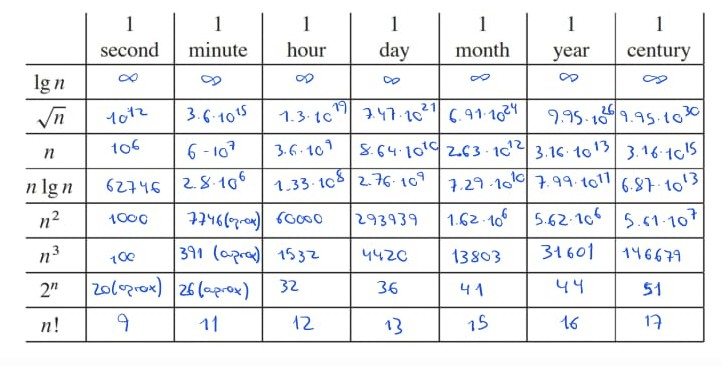
\includegraphics[scale=0.5]{Problem1_1}
    \centering
\end{figure*}


\refstepcounter{exercise}
\textbf{Exercise 2.1-1)}:\\
Note: Resolved using the logic of C, C++, Java, etc. while iterating over an array on a for
loop. Also the number that appears in \textcolor{ForestGreen}{green}, is the number being 
checked. The number or numbers that appears in \textcolor{Red}{red} are the numbers being 
moved.

\begin{center}
    \begin{tabular}{|c|c|}
    \hline
    \textbf{i} & \textbf{Array} \\
    \hline
    1) & [31, \textcolor{ForestGreen}{41}, 59, 26, 41, 58]\\
    2) & [31, 41, \textcolor{ForestGreen}{59}, 26, 41, 58]\\
    3) & [\textcolor{ForestGreen}{26}, \textcolor{Red}{31}, \textcolor{Red}{41}, 
          \textcolor{Red}{59}, 41, 58]\\
    4) & [26, 31, 41, \textcolor{ForestGreen}{41}, \textcolor{Red}{59}, 58]\\
    5) & [26, 31, 41, 41, \textcolor{ForestGreen}{58}, \textcolor{Red}{59}]\\
    \hline
    \end{tabular}
\end{center}

\refstepcounter{exercise}
\textbf{Exercise 2.1-2)}:\\
\textbf{Initialization}: The loop start getting the first number in the array. In spite of 
that, it has initialized to 0 the variable sum where the total sum will be stored. Due to 
that, the invariant holds the first number that will be added to sum.

\textbf{Maintenance}: On each iteration, the loop will hold only the index of the number 
that will be added, after add it, i will be incremented by 1, holding the next number (i + 1).

\textbf{Termination}: The loop will terminate when the 'n' elements of the array are added. In conclusion,
sum it's equivalent of say that $sum = \sum_{i = 1}^{n} A[i]$.
    
\refstepcounter{exercise}
\textbf{Exercise 2.1-3)}:\\
click this link to see the resolution \(\rightarrow \href{https://github.com/Graburr/Algorithms_CLRS_4ed_solutions/blob/main/chapter1/Getting_Started/2.1-3.cpp}
{\textcolor{blue}{resolution}}\)

\refstepcounter{exercise}
\textbf{Exercise 2.1-4)}:\\
\begin{algorithm}
\caption{Linear Search}\label{linearSearchID}
\begin{algorithmic}[1]
\Function{Linear-Search}{$A, n, x$}
    \For{$i \gets 1$ \textbf{to} $n$}
        \If {$ A[i] == x $} 
            \Return $i$
        \EndIf
    \EndFor
    \State \Return \textit{NIL}
\EndFunction
\end{algorithmic}
\end{algorithm}

\textbf{Initialization}: The loop start getting the first element of the array. 

\textbf{Maintenance}: On each iteration, the loop takes the next element (i + 1) and compare 
it with the value being search (x). If it's found return i, else, continue searching that 
value.

\textbf{Termination}: When all values are read, if x wasn't found in the array, it returns
NIL to indicate that no value was found on all the array.

\refstepcounter{exercise}
\textbf{Exercise 2.1-5)}:\\
\begin{algorithm}
\caption{ADD-BINARY-INTEGERS}\label{AddBinarySearchID}
\begin{algorithmic}[1]
\Function{ADD-BINARY-INTEGERS}{$A, B, n$}
    \State \textit{//Initialize array C with n values}
    \State \textit{carry} $\gets 0$ 
    \For {$i \gets 1$ \textbf{to} $n$}
        \State $c \gets A[i] + B[i]$
        \State $C[i] \gets c \mod 2$
        \State $carry \gets c \div 2$ \quad \textit{//Integer division}
    \EndFor
    \Statex
    \State $C[n] \gets carry$
    \State \Return \textit{C} \quad \textit{//Return the array C with the values}
\EndFunction
\end{algorithmic}
\end{algorithm}

\textbf{Initialization}: The loop starts with value of carry to 0, and getting the first 
bits of A and B.

\textbf{Maintenance}: On each iteration, the loop takes the next bits values of A and B.
Add these values and calculate the value to insert into C and the carry that could exists.

\textbf{Termination}: All values were added and store, now C[0:n - 1] with the result of 
the sum. To reach the n-th value, adds the last carry value on the position n.

\refstepcounter{exercise}
\textbf{Exercise 2.2-1)}:\\
Like the book says, \(\Theta\) notation is like saying "roughly proportional to \(n^2\) (for example), 
when \(n\) is large." In this case, we remove constants, so the remaining expression is 
\(n^3 + n^2 + n + 3\). The term with the highest exponent is \(n^3\), so at any moment:
\(n^3 \gg n^2 \gg n\). \\ 
\textbf{Solution}: \(\Theta(n^3)\).

\refstepcounter{exercise}
\textbf{Exercise 2.2-2)}:\\
\begin{algorithm}
\caption{SELECTION-SORT}\label{SelectionSortID}
\begin{algorithmic}[1]
\Function{SELECTION-SORT}{$A, n$}
    \For{$i \gets 1$ \textbf{to} $n - 1$}
        \State $ind\_small\_elm \gets i$
        \For{$j \gets i + 1$ \textbf{to} $n$}
            \If{$A[ind\_small\_elm] > A[j]$}
                \State $ind\_small\_elm \gets j$
            \EndIf
        \EndFor
        \State \Call{swap}{$A[i], A[ind\_small\_elm]$}
    \EndFor
\EndFunction
\end{algorithmic}
\end{algorithm}

The invairant is that on each iteration of extern for, it only takes 1 by 1 element. In the
inner for, also take all elemnts from i to n, and compare the value of the outter for
against the inner for to take the smaller elemnt.

When the algorithm arrives to the last element, all swaps ocurred and the last element will
be in the correct place.

The worst case happens when it must iterate on the outher for and also with al the elements
from i to n in the inner for. So it's: \(\frac{n*(n - 1)}{2}\). Thats mean that avoiding all
constants values, the solution is: \(\Theta(n^2)\).

The best case is not better because you have to check all values in the if, the only instruction
that is avoided is the instruction inside the if because the if won't be evaluated to true.
But that instruction is insignificant if \(n\) it's too big.

\refstepcounter{exercise}
\textbf{Exercise 2.2-3)}:\\
Depends on the value where is storage, if the \(x\) value is storage at the first position it
will take a constant value to search it. However, if the value is in the last element 
(worst case) it will spend \(constant * n\) time to find that value.

Averege case is suposing that it's in the middle of the array. The averegage is \(\frac{n}{2} = n\)
if \(n\) it's too big. 

Worst case as mentioned before is \(\Theta(n)\).

\refstepcounter{exercise}
\textbf{Exercise 2.2-3)}:\\
The only thing you could do is a preprocessing step to check if it's alredy sorted or nearly
to be sorted and then apply the algorithm who best fits when the best case was achieved.

\refstepcounter{exercise}
\textbf{Exercise 2.3-1)}:\\
\begin{figure*}[h]
    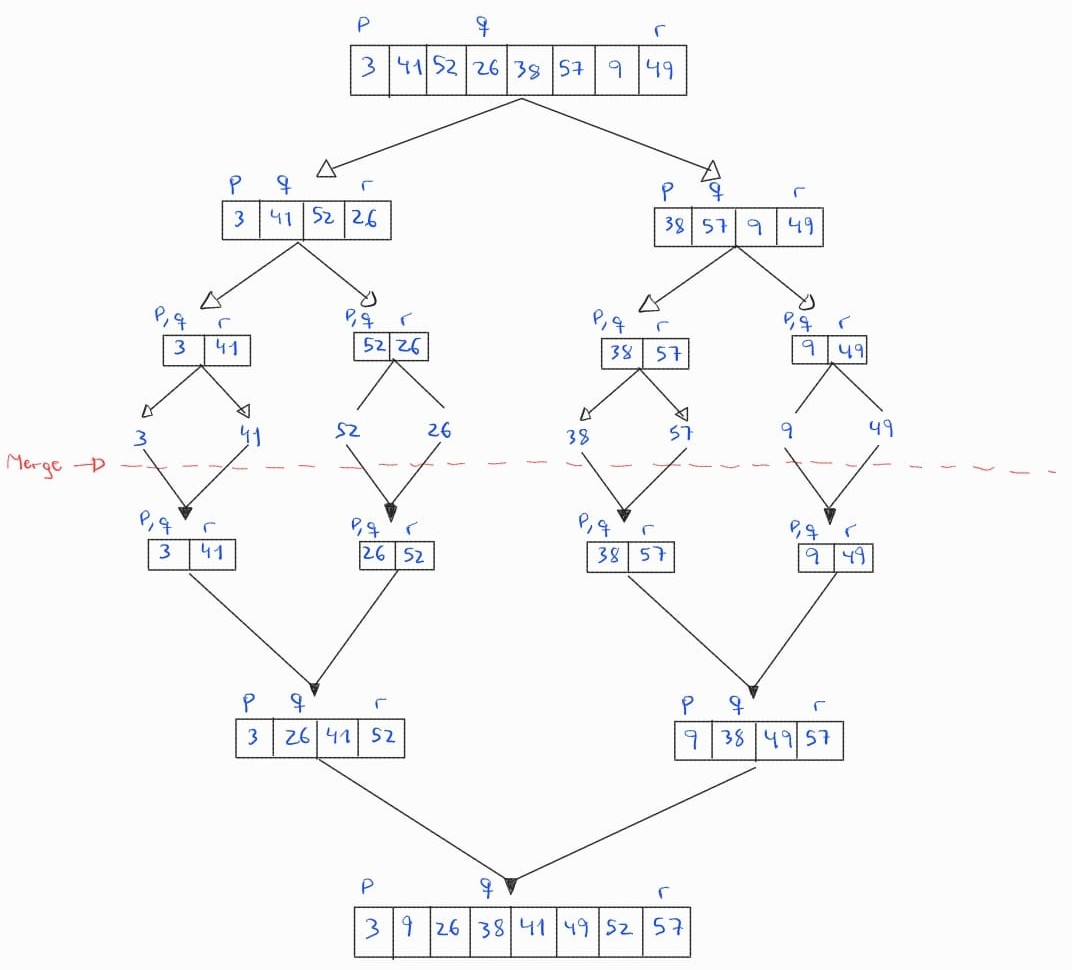
\includegraphics[scale=0.4]{Problem2_3_1.jpeg}
    \centering
\end{figure*}
\newpage

\refstepcounter{exercise}
\textbf{Exercise 2.3-2)}:\\
The "\textit{\textbf{if} \(p \neq r\)}" is not useful because \(p = 1\) and \(q > 1\), so the if
will be evaluated to true, and the return (the termination of recursion) will execute without
doing any recursion step.

\refstepcounter{exercise}
\textbf{Exercise 2.3-3)}:\\
\textbf{Initialization}: The loop starts obtaning the first element to insert it in the 
sorted array.

\textbf{Maintenance}: On each iteration, the loop insert 1 element of the left or right array,
then increment \textit{k} by 1, to insert on the next iteration the next value 1 by 1. The values
that will be inserted with the first loop in the best case is \textit{n - 1} where n is the
lenght of the subarray/array being sorted.

\textbf{Termination}: In one of the last 2 whiles, it will be inserted all remaining values
(could be values in the left or right array) until reach the nth values in the sorted array.

\refstepcounter{exercise}
\textbf{Exercise 2.3-4)}:\\
\textit{n = 2}
\[
T(2) = 2
\]
The solution given says that:
\[
T(2) = 2 * \log_2 2 = 2 \cdot 1 = 2
\]
Induction hypotesis:
\[
T(k) = k \cdot \log_2 k
\]
Where k is a power of 2. We want to demostrate that \textit{n = 2k}.
Use recurrence to calculate \(T(2k)\):
\[
T(2k) = 2T(k) + 2k \quad \rightarrow \quad T(2k) = 2 \cdot (k * \log_2 k) + 2k \quad \rightarrow
\quad T(2k) = 2k \cdot (\log_2 k + 1) \quad \rightarrow \quad T(2k) = 2k \cdot \log_2 2k
\]
As we mentiones before, replacing \textit{n = 2k}, we conclude that the induction hypotesis
is correct \textbf{\(n \cdot \log_2 n\)}

\refstepcounter{exercise}
\textbf{Exercise 2.3-5)}:\\
\begin{algorithm}
    \caption{INSERTION-SORT-RECURSIVE}\label{InsertionSortRecursiveID}
    \begin{algorithmic}[1]
        \Function{INSERTION-SORT-RECURSIVE}{$A, n$}
            \If{\(n == 0\)}  
                \Return
            \EndIf
            \State \Call{INSERTION-SORT-RECURSIVE}{$A, n - 1$}
            \State \textit{key} $\gets$ \textit{A[n]}
            \State $i \gets n - 1$
            \While {$i \geq 0$ \textbf{and} $A[i] > key$}
                \State $A[i + 1] \gets A[i]$
                \State $i \gets i - 1$
            \EndWhile
            \State $A[i + 1] \gets key$
        \EndFunction
    \end{algorithmic}
\end{algorithm}

\newpage
\refstepcounter{exercise}
\textbf{Exercise 2.3-6)}:\\
\begin{algorithm}
    \caption{BINARY-SEARCH}\label{BinarySearchID}
    \begin{algorithmic}[1]
        \Function{BinarySearch}{$A, x, l, n$}
            \If {\(l > n\)}
                \Return
            \EndIf
            \State \textit{mid} \(\gets\) \(l + n / 2\)
            \If {\(A[mid] > x\)}
                \State \Call{BinarySearch}{$A, x, l, mid - 1$}
            \ElsIf {\(A[mid] < x\)}
                \State \Call{BinarySearch}{$A, x, mid + 1, r$}
            \Else 
                \quad \Return \textit{mid}
            \EndIf
        \EndFunction
    \end{algorithmic}
\end{algorithm}

\refstepcounter{exercise}
\textbf{Exercise 2.3-7)}:\\
You can't use binary search because while you are sorting most part of the time, it won't
be that value in the sorted array. Maybe you should make a variation of binary search to 
find out in which direction has less difference betwen the number being search and then
you should move all values 1 position to right and insert in the new position.

On worst case, imagine that the worst value is at the least position, you should move
n items to the right + n / 2 that cost to search all the. So it's  \(n \cdot \frac{n}{2} = \Theta(n^2)\)

\refstepcounter{exercise}
\textbf{Exercise 2.3-8)}:
\begin{algorithm}
    \caption{FIND-SUM-TWO-ELEMENTS}\label{FindSumTwoElementsID}
    \begin{algorithmic}[1]
        \Function{FindSumTwoElements}{$S, n, x$}
            \State \Call{MergeSort}{S, 0, n - 1} \quad \textit{//\(\Theta(n * log n)\)}
            \State \( i \gets 0 \)
            \State \( j \gets n - 1 \)
            \While {\( i < j \)} \quad \textit{//\(\Theta(n)\)}
                \If {\( S[i] + S[j] = x \)}
                    \State \Return \( i, j \)
                \ElsIf {\( S[i] + S[j] < x \)}
                    \State \( i \gets i + 1 \)
                \Else
                    \State \( j \gets j - 1 \)
                \EndIf
            \EndWhile
            \State \Return \textit{No pair found}
        \EndFunction
    \end{algorithmic}
\end{algorithm}

\underline{\large{Problems of page 45}}\\
\\
\refstepcounter{exercise}
\textbf{Exercise 2-1)}:\\
\textbf{a)} The number of arrays to be sort are \(\frac{n}{k}\), where \textit{n} is the
number of elements in the original array and \textit{k} the number of elements to be sorted on
\textit{insertion sort}. Due to that, on the worst case it should be sorted \(\frac{n}{k}
\cdot k^2 \quad \rightarrow n \cdot k = \Theta(n \cdot k)\).

\textbf{b)} The recursion will be called until reach \(\frac{n}{k}\) elements on a subarray.
Hence it won't be called recursively until \(\log_2 n\) (when only 1 element is left). 
Due to that the number of recursions are delimited by \(\log_2 \frac{n}{k}\). Finally in the
worst case when only is left the first 2 subarrays, it will take \textit{n} iterations to
sort it. Due to that, we explain why it's true the expresion \(\Theta(n \cdot \log_2 \frac{n}{k})\).

\textbf{c)}  
\[
\Theta\left(n \cdot k + n \cdot \log_2 \frac{n}{k}\right) = \Theta(n \cdot \log_2 n)
\]
\[
\Theta(n \cdot k) = \Theta(n \cdot \log_2 n) \quad \rightarrow \quad k = \Theta(\log_2 n)
\]
\[
\Theta\left(n \cdot \log_2 \frac{n}{k}\right) = \Theta(n \cdot \log_2 n) \quad 
\text{//Substituting } k = \Theta(\log_2 n)
\]
\[
\Theta\left(n \cdot \log_2 \frac{n}{\log_2 n}\right) = \Theta(n \cdot \log_2 n) - \Theta(n \cdot \log_2 \log_2 n)
\quad \text{//Dominant term is  \(\Theta(n \cdot \log_2 n)\)}
\]
In conclusion, the biggest posible value which both variants of Merge Sort have the same result
is for \(k = \Theta(\log_2 n)\).

\textbf{d)}
You should see in which value it's better use one algorithm or another to sort and combine
the 2 algorithms. As we saw in the section c, this k value is calculated applying that formula.

\refstepcounter{exercise}
\textbf{Exercise 2-2)}:\\
\textbf{a)} Do you need to prove that on each iteration, of the inner for 1 element is being
moved and it remains on all iterations. In addition to that, you must prove that on the extern
for loop it's being incremented by 1.

\textbf{b) Initialization}: The loop starts taking the most right element on the array.
So the invariant is that take 1 element at a time.

\textbf{Maintenance}: Loop takes on each iteration an element, compare with the left hand
elemnt and if it's smaller than the left hand element, swap both elements. The loop invariant
remains as Initialization because on each iteration only 1 element is being checked with
another one. After that check, on the next iteration is taken the next left element.

\textbf{Termination}: When this for ends, there are a number of elements equals to \textit{i} 
(extern for) that are sorted in the lowest positions of the array.

\textbf{c)} As I said before, on each time that the inner for loop ends, 1 value is sorted.
Hence when the extern for loop ends, all values will be sorted on the right position and it's
proved the inequality.

\textbf{d)} Both have the same worst-case running time (\(\Theta(n^2)\)). But Insertion
Sort is usually better on the averegage cases because it does less swaps and usually spends
\(\Theta(n)\) on sort an array. On the other hand, Bubble Sort always spend \(Theta(n^2)\)
to sort the array. 

\refstepcounter{exercise}
\textbf{Exercise 2-3)}:\\
\textbf{a)} \(\Theta(n)\) because it has to take all values of the array \textit{A} and 
add it to \(x \cdot p\).

\textbf{b)}
\begin{figure*}[h]
    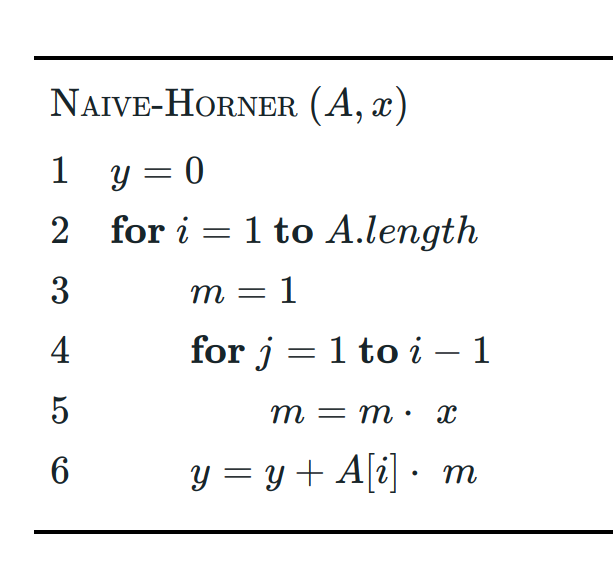
\includegraphics[scale=0.3]{Problem2_3_b}
    \centering
    \caption{Resolution extracted from \href{https://atekihcan.github.io/CLRS/02/P02-03/}
    {https://atekihcan.github.io/CLRS/02/P02-03/} I was lazy of do that hehehe.}
\end{figure*}

\textbf{c)}
For \underline{Maintenance}:
\[
y = a_i + x \sum_{k=0}^{n-(i+1)} a_{k+i+1} x^k
\]

\[
= a_i x^0 + \sum_{k=0}^{n-i-1} a_{k+i+1} x^{k+1}
\]

\[
= a_i x^0 + \sum_{k=1}^{n-i} a_{k+i} x^k
\]

\[
= \sum_{k=0}^{n-i} a_{k+i} x^k.
\]

The loop \underline{terminates} at i = -1:

\[
= a_i x^0 + \sum_{k=0}^{n-i-1} a_{k+i+1} x^{k+1} = \sum_{k=0}^{n-i} a_{k+i} x^k.
\]

\refstepcounter{exercise}
\textbf{Exercise 2-4)}:\\
\textbf{a)} Inversions are: (2, 1), (3, 1), (8, 6), (8, 1), (6, 1)

\textbf{b)} if the set is sor in ascending order, it won't be 0 inversions in the set.

\textbf{c)} Both of them are \(\Theta(n^2)\) because you have to take 1 value from the most
right position and compare if it's less than the i value (left one) on the array.

\textbf{d)}
\begin{algorithm}
    \caption{INVERSIONS}\label{InversionID}
    \begin{algorithmic}[1]
        \Function{Inversions}{$A, p, r$}
            \State \textit{//On the else of the first while of Merge, add: Print(L[i], R[j])}
        \EndFunction
    \end{algorithmic}
\end{algorithm}


\subsection{Caharcerizing Running Times}
\setcounter{exercise}{0}

\refstepcounter{exercise}
\textbf{Exercise 3.1-1)}:\\
We could do the same with saying that \textit{k} is a multiple of 2. The left subarray
has the biggests numbers, and the right one have the lowest numbers. If we want to move the
biggests numbers to the right subarray, we should move \textit{n / 2} numbers and then another
\textit{n / 2} to the left to move the lowest one at the begginig. Finally we have that
we should move \(\frac{n}{2} \cdot \frac{n}{2} = \frac{n^2}{4} = \Omega(n^2)\)

\refstepcounter{exercise}
\textbf{Exercise 3.1-2)}:\\
The extern for loop, executes in the worst case \textit{n - 1}  times. The inner loop, executes 
\textit{i + 1} to \textit{n} times. As mentioned before, the worst case is for i = 0, then
it will be executed \textit{n - 1} times. In conclusion, the wors case is \((n - 1) \cdot 
(n - 1) = O(n^2)\).

On the other hand, supose that the array is divided in 2 subarrays, the left for the higer 
values and the right for the lower ones. Althought, the extern for must iterate over all
elements, so the better case is the same as the worst (\textit{n - 1}). Then the inner loop
is the same as the worst case. The only thing that executes n/2 times is the instruction 
inside the if and the swap. These operations are constant operations. In conclusion, the
lower bound of the asymptotic behaviour is \((n - 1) \cdot (n - 1) = \Omega(n^2)\)

\textbf{\(O(n^2) = \Omega(n^2) = \Theta(n^2)\)}

\refstepcounter{exercise}
\textbf{Exercise 3.1-3)}:\\
Consideramos un array \(A\) de tamaño \(n\), dividido en tres partes:
\begin{itemize}
    \item Primera parte: Las primeras \(\alpha n\) posiciones contienen los \(\alpha n\) valores más grandes.
    \item Segunda parte: Las siguientes \((1 - 2\alpha)n\) posiciones son la parte media.
    \item Tercera parte: Las últimas \(\alpha n\) posiciones contienen los \(\alpha n\) valores más grandes después de ordenar.
\end{itemize}
El número total de movimientos es:
\[
\text{Movimientos totales} = \alpha(1 - 2\alpha)n^2.
\]
Para que el argumento tenga sentido, necesitamos que \(0 < \alpha < \frac{1}{2}\).

Maximizamos la función:
\[
f'(\alpha) = 1 - 4\alpha = 0 \quad \Rightarrow \quad \alpha = \frac{1}{4}.
\]

El número total de movimientos es:
\[
\frac{1}{4} \cdot \frac{1}{2} n^2 = \frac{1}{8}n^2.
\]
Por lo tanto, el tiempo de ejecución en el peor caso es \(\Theta(n^2)\).

\refstepcounter{exercise}
\textbf{Exercise 3.2-1)}:
\[
0 \leq c_1g(n) \leq f(n) \leq c_2g(n) = \Theta 
\]
Prove that \(\max \{f(n), g(n)\} = O(f(n) + g(n)) \quad \Rightarrow \quad \max\{f(n),g(n)\}
\leq c_2 \cdot (f(n) + g(n))\).

If the max value is \textit{f(n)}, then we have \(f(n) \leq c_2 \cdot (f(n) + g(n))\).
Also if the max value is \textit{f(n)}, then we have \(g(n) \leq c_2 \cdot (f(n) + g(n))\)
If \(c_2 = 1\), and \(n \geq n_0\), the result is \(\max \{f(n), g(n)\} = O(f(n) + g(n))\).

Prove that \(\max \{f(n), g(n)\} = \Omega(f(n) + g(n)) \quad \Rightarrow \quad \max\{f(n),
g(n)\} \geq c_1 \cdot (f(n) + g(n))\).

If the max value is \textit{f(n)}, then we have \(f(n) \geq c_1 \cdot (f(n) + g(n))\).
Also if the max value is \textit{f(n)}, then we have \(g(n) \geq c_1 \cdot (f(n) + g(n))\)
If \(c_1 = \frac{1}{2}\), and \(n \geq n_0\), the result is \(\max \{f(n), g(n)\} = \Omega
(f(n) + g(n))\).

\textbf{In conclusion}: \(\max \{f(n), g(n)\} = O(f(n) + g(n)) = \Omega(f(n) + g(n)) =
\Theta(f(n) + g(n))\) for \(c_1 = \frac{1}{2}\) and \(c_2 = 1\).

\refstepcounter{exercise}
\textbf{Exercise 3.2-2)}:\\
It's meaningless because de O notation defines asymptoticaly, the upper bound of f(n). This 
not mean \textit{"Is at least \(O(n^2)\)"} because it's only in the worst possible scenario.
Althought, we need to define the ower bound, for example the asymptotic lower bound is 
\(\Omega(n)\) that it's less than \(O(n^2)\). Hence we can't say \textit{"At least"} due to
it could spend some value betwen \(O(n^2)\) on the worst case or \(\Omega(n)\) in the best
cases.

\refstepcounter{exercise}
\textbf{Exercise 3.2-3)}:\\
With the properties of the powers, we have: 
\[
2^{n + 1} = 2^n \cdot 2^1 = O(\max\{2^n, 2^1\}) = O(2^n)
\]
The second one is wrong, because with the properties we can't remove the n there, so it
should be \(O(2^{2n})\).

\refstepcounter{exercise}
\textbf{Exercise 3.2-5)}:
\[
0 \leq c_1g(n) \leq g(n) \leq c_2g(n) = \Theta(g(n)) 
\]
\[
\Omega(g(n)) = c_1g(n) \leq g(n) \quad c_1 = \frac{1}{2} \text{ and } n \geq n_0
\]
\[
O(g(n)) = c_2g(n) \geq g(n) \quad c_2 = 2 \text{ and } n \geq n_0
\]

\refstepcounter{exercise}
\textbf{Exercise 3.2-6)}:\\
All the values of the time spent by the algorithm, will be on \(\Omega(g(n)) = g(n)
= O(g(n))\) if \(\Theta(g(n))\). Also we know that \(o(g(n)) > O(g(n))\) and 
\(\omega(g(n)) < \Omega(g(n))\), so they won't have values in common.

\refstepcounter{exercise}
\textbf{Exercise 3.2-7)}:\\
\(\Omega(g(n, m)) = \{ f(n, m)\) : if there exists a constant \textit{c}, \(n_0\) and \(m_0\) 
such that \(cg(n, m) \leq f(g, m)\) for all \( n \geq n_0\) or \(m \geq m_0\) and \(c > 0 \}\).

\(\Theta(g(n, m)) = \{ f(n, m)\) if there exists a constant \(c_1\), \(c_2\), \(n_0\) and 
\(m_0\) such that \(0 \leq < c_1g(n, m) \leq g(n, m) \leq c_2g(g, m)\) for all \(n \geq n_0\)
or \(m \geq 0\) and \(c_1 > 0\), \(c_2 > 0 \}\).

\refstepcounter{exercise}
\textbf{Exercise 3.3-1)}:\\
\textit{f(n)} is monotically increasing because there is an \(f(m) \leq f(n)\). For \textit{g(n)}
it's the same. Then we have: 
\[
f(m_1) \leq f(n_1) + g(m_2) \leq g(n_2) \quad \Rightarrow f(m_1) + g(m_2) \leq f(n_1) + g(n_2)
\]
Demostrate \(f(g(n))\):
\[
f(g(m)) \leq f(g(n)) \quad m \leq n
\]
Demostrate \(f(n) \cdot g(n)\) are non negative for an \(n_1 > 0, n_2 > 0, m_1 < n_1 and m_2 < n_2\) 
\[
f(m_1) * g(m_2) \leq f(n_1) * g(n_2)
\]

\refstepcounter{exercise}
\textbf{Exercise 3.3-2)}:
\[
\lfloor \alpha n \rfloor = \alpha n \quad \quad \lceil (1 - \alpha)n \rceil = (1 - \alpha)n
\]
\[
\alpha n + (1 - \alpha)n = n(\alpha + 1 - \alpha) = n
\]

\refstepcounter{exercise}
\textbf{Exercise 3.3-3)}:\\
Applying the properties of exponentials, we have
\[
(n + o(n))^k = n^k + o(n^k) \quad \Rightarrow \quad \Theta(\max \{n^k, n^k\}) = \Theta(n^k)
\]
With the property of ceil and floor, we know \(\lceil n \rceil^k \leq n^k \leq \lfloor n 
\rfloor^k\), the problem says \(\Theta(n^k) = n^k\)

\refstepcounter{exercise}
\textbf{Exercise 3.3-4)}:
\begin{enumerate}[label=\alph*)]
    \item Equation \(a^{\log_b c} = c^{\log_b a}\)
    \[
    \log_b c = x \quad \quad \log_b a = y
    \]
    \[
    a^x = (b^y)^x \quad \Rightarrow \quad a^{\log_b c} = b^{yx}
    \]
    Use the relation \(c = b^x\)
    \[
    c^y = (b^x)^y \quad \Rightarrow \quad c^{\log_b a} = b^{xy}
    \]
    \[
    a^{\log_b c} = b^{yx} = c^{\log_b a}
    \]
    \newpage
    \item Demostrate equations 3.26, 2.27 y 3.28.

    3.26) 
    \[
    n! = \sqrt{2\pi n} * \left(\frac{n}{e}\right)^n + 1 \quad \Rightarrow \quad (2\pi n)^
    \frac{1}{2} * \left(\frac{n}{e}\right)^n + 1
    \]
    Removing the constant values that are \(2, \pi, e, 1\), the reamining values are:
    \(n^{\frac{1}{2}} \cdot n^n = o(n^n)\).

    3.27)
    \[
    n! \approx \sqrt{2 \pi n} \left(\frac{n}{e}\right)^n.
    \]
    Prove \( n! = \omega(2^n) \), that's mean:
    \[
    \frac{n!}{2^n} \to \infty.
    \]

    Dividiendo por \( 2^n \),
    \[
    \frac{n!}{2^n} \approx \sqrt{2\pi n} \left(\frac{n}{2e}\right)^n.
    \]
    For a bigger value of \( n \) , \( \frac{n}{2e} > 1 \), the term tends to infinity.
    We can conclude that
    \[
    n! = \omega(2^n).
    \]
    \item \(\log_2(\Theta(n)) = \Theta(\log_2 n)\)
    \[
    \log_2(c_1 \cdot n) \leq \log_2(f(n)) \leq \log_2(c_2 \cdot n) \quad \Rightarrow \quad
    \log_2 c_1 + \log_2 n \leq \log_2(f(n)) \leq \log_2 c_2 + \log_2 n.
    \]
    \(\log_2 c_1\) and \(\log_2 c_2\) are constants. Hence we have: \(\log_2(f(n)) = 
    \Theta(\log_2 n) \quad \Rightarrow \quad \log_2(\Theta(n)) = \Theta(\log_2 n)\)
\end{enumerate}

\refstepcounter{exercise}
\textbf{Exercise 3.3-5)}:\\
As we saw, \(\lceil \log_2 n \rceil! = \log_2 n!\) applying the formula 3.28, we have that
\(\log_2 n = \Theta(n \log_2 n)\). In conclusión, it's polinomially bounded.

\(\lceil \log_2{\log_2 n} \rceil! = \log_2{\log_2 n} = \log_2{\Theta{n * \log_2 n}}\)
with that we can show that is \textbf{not} polinomally bounded.

\refstepcounter{exercise}
\textbf{Exercise 3.3-6)}:\\
for the definition, we know \(\log_2^* n < 5\) (rarely will be upper to 5). If we supose that
takes the value of \(n = 2^{65536} = 10^{\frac{65536}{\log_2 10}} \approx 10^{19.728}\) The result of
\(\log_2^* 10^19.728 = 5\) for example, then we have \(\log_2 5 \approx  2.322\).

On the other hand, for the same \textit{n} value, we have \(\log_2 10^19.728 \approx 65.535\)
then looking the table, Applying the logarithm iteratively, we can see:
\begin{enumerate}
    \item \(\log_2 65.535 \approx 6.02\).
    \item \(\log_2 6.02 \approx 1.37\)
    \item \(\log_2 1.37 \approx 0.45\)
\end{enumerate}
Because we could apply 3 times the iteration, \(\log_2^*(\log_2 n) = 3\).
\textbf{In conclusion}, \(\log_2^*(\log_2 n) >\) \(\log_2(\log_2^* n)\)

\refstepcounter{exercise}
\textbf{Exercise 3.3-7)}:\\
Substitute \(\phi = \frac{1 + \sqrt{5}}{2}\) in \(x^2 = x + 1\).
\[
\left(\frac{1 + \sqrt{5}}{2}\right)^2 = \frac{1 + \sqrt{5}}{2} + 1 \quad \Rightarrow \quad
\frac{3 + \sqrt{5}}{2} = \frac{3 + \sqrt{5}}{2}  
\]
With the \(\widehat{\phi}\) is do the same procedure.

\refstepcounter{exercise}
\textbf{Exercise 3.3-9)}:\\
supose \(\log_2 k = \log_2 n\), then operating we have: 
\[
\frac{k * \log_2 n}{\log_2 n} = \Theta\left(\frac{n}{\log_2 n}\right) \quad \Rightarrow \quad
k = \Theta\left(\frac{n}{\log_2 n}\right)
\]

\subsection{Divide and Conquer}
\setcounter{exercise}{0}

\refstepcounter{exercise}
\textbf{Exercise 4.1-1)}:\\
\(T(n) = 8T(\lfloor\frac{n}{2}\rfloor + \Theta(1))\). As mentioned before, the ceil and floor
doesn't matter on anylizing algorithms when \textit{n} is too big. Due to that, the result
is the same \(T(n) = \Theta(n^3)\).

\refstepcounter{exercise}
\textbf{Exercise 4.1-2)}:\\
The length of the matrix that you pass as a fourth parameter, now it should be \(k * n\), for
bigger values of n and k, is the same as says, \(T(n) = 8T(\frac{k * n}{2}) + \Theta(1)\).
Now the result is \(T(n) = \Theta(k * n^3)\). 

The second option is the same as the first one. Inconclusion any of them is asymptoticaly
faster than the other one, both of them have the same speed.

\refstepcounter{exercise}
\textbf{Exercise 4.1-3)}:\\
Now is \(\Theta(n^2)\) the driving function because you need to combine the solutions.
Then \(T(n) = 8T(\frac{n}{2}) * \Theta(n^2)\). Applying the master theorem, \(n^{\log_2 8}
= 3\), case 1 applies again. \(f(n) = O(n^{3 - \epsilon})\) for any positive \(\epsilon \leq
1\)

\refstepcounter{exercise}
\textbf{Exercise 4.1-4)}:\\
Exercise resolved in cpp on the file \href{https://github.com/Graburr/Algorithms_CLRS_4ed_solutions/blob/main/chapter1/Divide_%26_Conquer/MatrixAddRecursive.cpp}
{\textcolor{blue}{MatrixAddRecursive.cpp}} (click on that to go to the file).

The cost of that algorithm is \(T(n) = 4T(\frac{n}{2}) + \Theta(1)\). The whatershed function
is: \(n^{\log_2 4} = n^2\). We have that \(f(n) = O(n^{2 - \epsilon})\) for a positive
\(\epsilon <= 2\). So we are on the case 1, the solution is: \(T(n) = \Theta(n^2)\).

The case we have: \(T(n) = 4T(\frac{n}{2}) + \Theta(n^2)\). The whatershed function is: 
\(n^{\log_2 4} = n^2 = f(n) = \Theta(n^2)\). Applying case 2, the solution is: \(T(n) = 
\Theta(n^2 \log_2 n)\).

\refstepcounter{exercise}
\textbf{Exercise 4.2-1)}:
\begin{align*}
    S_1 &= 8 - 2 = 6 \\ S_2 &= 1 + 3 = 4 \\ S_3 &= 7 + 5 = 12 \\ S_4 &= 4 - 6 = -2 \\ 
    S_5 &= 1 + 5 = 6 \\ S_6 &= 6 + 2 = 8 \\ S_7 &= 3 - 5 = -2 \\ S_8 &= 4 + 2 = 6 \\
    S_9 &= 1 - 7 = -6 \\ S_{10} &= 6 + 8 = 14   
\end{align*}

The P values are:
\begin{align*}
    P_1 &= 1 * 6 = 6 \\ P_2 &= 4 * 2 = 8 \\ P_3 &= 12 * 6 = 72 \\ P_4 &= 5 * -2 = -10 \\
    P_5 &= 6 * 8 = 48 \\ P_6 &= -2 * 6 = -12 \\ P_7 &= -6 * 14 = -84
\end{align*}
\newpage
The result of the matrix is:
\begin{align*}
    C_{11} &= 48 - 10 - 8 - 12 = 18 \\ C_{12} &= 6 + 8 = 12 \\
    C_{21} &= 72 - 10 = 62 \\ C_{22} &= 48 + 6 -72 + 84 = 66
\end{align*}
\[
C =
\begin{bmatrix}
    18 & 12 \\
    62 & 66
\end{bmatrix}
\]

\refstepcounter{exercise}
\textbf{Exercise 4.2-2)}:\\
You can find the pseudocode on that website (it's not mine, it's from another one):
\href{https://atekihcan.github.io/CLRS/04/E04.02-02/}{https://atekihcan.github.io/CLRS/04/E04.02-02/}.

I implemented it in C++ using the code of exercise 4.1-4 (adding the function to substract matrices).
You can find the result of that code clicking there: \href{https://github.com/Graburr/Algorithms_CLRS_4ed_solutions/blob/main/chapter1/Divide_%26_Conquer/StrassensAlgorithm.cpp}
{\textcolor{Blue}{StrassensAlgorithm.cpp}}.

\refstepcounter{exercise}
\textbf{Exercise 4.2-3)}:\\
The largest \textit{k} should be 7 because it's the number os time that the algorithm is 
called recursively. Also we can prove that applying the case 1 of the master theorem to 
\(T(n) = aT\left(\frac{n}{2}\right) + \Theta(1)\) where \(a = k\) for the reasons explained 
at the beggining.

\refstepcounter{exercise}
\textbf{Exercise 4.2-4)}:\\
Strassen's alrogithm is better that the navie way of multyplying matrices.

Then we know that the Strassen's algorithm spends \(\Theta(n^{\log_2 7}) = \Theta
(n^{2.8})\). Then applying the \textit{68 x 68} where \(n = 68\), applying this method the
amount of time required is \(68^{2.8} = 135215\). For \(n = 70\), the result is \(70^{2.8}
 = 146647\). The last one is \(n = 72\) and the result is \(72^{2.8} = 158683\). The Strassen's
alrogithm is a little bit inneficienter than the Pan ways to multiply this particular
matrices. 

\refstepcounter{exercise}
\textbf{Exercise 4.2-6)}:\\
It will be done using block matrices (join 2 differents matrices in 1 matrice to operate).
Then the solution will be \(M^2 \quad \Rightarrow \quad O((2n)^\alpha) = O(n^\alpha)\).

\refstepcounter{exercise}
\textbf{Exercise 4.7-2)}:\\
To check that is polynominal-growt we need to proof \(\frac{f(n)}{n^c}\) for \(f(n) = n^2\).
We need to check if  there exists such a constat c that: \(\frac{n^2}{n^c} = n^{2 - c}\).
In that case for c = 3 we have: \(\frac{n^2}{n^3} = n^-1 = \frac{1}{n}\). Since \(\frac{1}{n}\)
is bounded for any \(n \geq 1\), \(f(n) = n^2\) satisfies the polynominal growth condition.

On the other hand we will apply the same argumentation. we need to check if there exists any
\(c\) for \(\frac{2^n}{n^c}\). We supose the case of \(\lim_{n \to \infty} \frac{2^n}{n^c}\).
In that case \(2^n\) growth exponentialy to the \(\infty\) while \(n^c\) growth polynomially.
Hence the exponentialy is not bounded and \(2^n\) does not satisfies the polynominal-growth.

\refstepcounter{exercise}
\textbf{Exercise 4.7-3)}:\\
If \( n \) tends to \( \infty \), the smallest possible value of \( f(n) \) will be 0, 
assuming it has a negative exponent. On the other hand, if \( f(n) \) is a polynomial
function like \( n^2 \), all values will be well-defined because it satisfies the 
polynomial-growth condition.

\refstepcounter{exercise}
\textbf{Exercise 4.7-4)}:\\
As explained before \(2^n\) doesn't satisfies the polinominal-growth condition.

To proof \(f(\Theta(n)) = \Theta(f(n))\) we need a constant \textit{c} that scales in the 
same asymptotic way. In that case: \(f(nc) = 2^{nc} = (2^n)^c = \Theta(f(n))\). So this is 
a valid example.

\refstepcounter{exercise}
\textbf{Exercise 4.7-5)}:
\begin{enumerate}[label=\alph*)]
    \item \(a_1 = a_2 = a_3 = 1\), \(b_1 = 2\), \(b_2 = 3\), \(b_4 = 6\).
    We need to find a p value that \(\left(\frac{1}{2}\right)^p + \left(\frac{1}{3}\right)
    ^p + \left(\frac{1}{6}\right)^p = 1\). For \(p = 0\), the result is 3. for \(p = 1\), 
    the result is: \(p = 0.9999...\). Then we know that \(0 < p < 1\). \(f(x) = n\log_2 n\)

    \begin{align*}
        T(n) &= \Theta\left(n^p\left(1 + \int_{1}^{n}\frac{f(x)}{x^{p + 1}}\,\mathrm{d}x \right)\right) \\
        &= \Theta\left(n^p\left(1 + \int_{1}^{n}x^{-p}\log_2 x\,\mathrm{d}x \right)\right) \\
        &= 1 + \frac{n^{1 - p}\log_2 n}{1 - p} - \frac{n^{1 - p}}{(1 - p)^2}
    \end{align*}
    For \(p = 1\) we see the biggest order is \(T(n) = \Theta(n\log_2 n)\).
\end{enumerate}

\subsection{Probabilistic Analysis and Randomized Alrogithms}


\setcounter{exercise}{0}
Note: Most exercises of this part weren't done because it wasn't my scope of understanding
that book. Anyway, I just suck at learning it and I dont have too much free time to
roll up my sleves and learn that perfectly. Maybe in the future I will try this again.

\refstepcounter{exercise}
\textbf{Exercise 5.1-1)}:\\
You know who is better because best starts on 0, that is the lees rank that u can achieve.
The biggest rank is bound at the upper with a maximum score of \textit{n}. Betwen on that 
interval of scores you can index eassly each worker by the score he got. 

\refstepcounter{exercise}
\textbf{Exercise 5.1-2)}:\\
An imlementation could be multiply a for the value that was got by \textit{Random(0, 1)}
and then make another math operation with b for example to introduce aleatority and give
as a result the number between a and b. That operations could be:
\(a + \lfloor(Random(0, 1) \cdot (b - a + 1))\rfloor\) That would give us a number between
[0, b - a + 1] and then adding a, we take a value between [a, b].

The expected running time is \(O(1)\).

\refstepcounter{exercise}
\textbf{Exercise 5.1-3)}:\\
We see the 2 posible values that exists with p and 1 - p are:
\begin{align*}
    P(00) &= (1 - p)(1 - p), \\
    P(01) &= (1 - p)p, \\
    P(10) &= p(1 - p), \\
    P(11) &= p p.
\end{align*}

01 and 10 happends with the same probability. If we have 01 we return 0. On the other hand
if we have 10 return 1. If neither of that values, keep trying until get 1 of these values.

\newpage
\begin{algorithm}
\caption{Generación de bit imparcial a partir de BIASED-RANDOM}
\begin{algorithmic}
    \Procedure{Unbiased-Random}{}
        \While{true}
            \State first $\gets$ BIASED-RANDOM()
            \State second $\gets$ BIASED-RANDOM()
            
            \If{first = 0 \textbf{and} second = 1}
                \State \Return 0
            \ElsIf{first = 1 \textbf{and} second = 0}
                \State \Return 1
            \EndIf
        \EndWhile
    \EndProcedure
\end{algorithmic}
\end{algorithm}

Running time is \(\frac{2}{2p(1 - p)} = \frac{1}{p(1 - p)} = O\left(\frac{1}{p(1 - p)}\right)\)

\refstepcounter{exercise}
\textbf{Exercise 5.2-1)}:\\
First of all we will use the same indicator random variable as mentioned in the book few 
pharagraphs before. The probability of being hired is \(\frac{1}{n}\) \textit{from 1 to n - 1},
That's mean because it's presented in a random order, it could be someone before you that
have better scores and he will be hired instead of you. 

To hire exactly n times, its \(\frac{1}{n!}\) because there is n permutations where you hire
everyone but only one of them is correct.

\refstepcounter{exercise}
\textbf{Exercise 5.2-2)}:\\
\(\frac{(n - 1)(n - 2)!}{n!}\) There is n - 1 positions to place the best candidate and
also you have n - 2 possibilities of place 2 person to hire them at the same time.

\refstepcounter{exercise}
\textbf{Exercise 5.2-3)}:\\
Let \( X = \sum_{i=1}^{n} X_i \), where \( X_i \) is the value of the \( i \)-th die. We use indicator random variables \( I_i(k) \), which take the value 1 if die \( i \) shows the value \( k \), and 0 otherwise. Then we can write:

\[
X_i = \sum_{k=1}^{6} k \cdot I_i(k)
\]

The expected value of \( X_i \) is:

\[
E[X_i] = E\left[ \sum_{k=1}^{6} k \cdot I_i(k) \right] = \sum_{k=1}^{6} k \cdot E[I_i(k)]
\]

Since \( E[I_i(k)] = \frac{1}{6} \), we get:

\[
E[X_i] = \sum_{k=1}^{6} k \cdot \frac{1}{6} = \frac{1}{6} (1 + 2 + 3 + 4 + 5 + 6) = 3.5
\]

Now, the expected value of \( X \) is:

\[
E[X] = E\left[ \sum_{i=1}^{n} X_i \right] = \sum_{i=1}^{n} E[X_i] = n \cdot 3.5
\]

\refstepcounter{exercise}
\textbf{Exercise 5.2-5)}:\\
\(X_i = I{customer gets his own hat}\). Probability of customer \textit{i} recieves his 
own hat is \(E[X_i] = Pr{I} = \frac{1}{n}\).

\[
E[x_i] = E \left[\sum_{i = 1}^{n} X_i\right] = \sum_{i = 1}^{n} E[X_i] = \sum_{i = 1}^{n} 
\frac{1}{n} = \frac{n}{n} = 1
\]
The number of costumers that receives his own hat is 1.

\refstepcounter{exercise}
\textbf{Exercise 5.2-6)}:\\
\(X_ij = I{an inversion was found}\). Probability of the inversion \textit{ij} to be found
is \(E[X_ij] = Pr{I} = \frac{1}{2}\). Number of inversions is:
\[
E[X_{ij}] = E \left[\sum_{1 \leq i \leq j \leq n}^{n} X_{ij}\right] = \sum_{1 \leq i \leq j
\leq n}^{n} E[X_{ij}] = \frac{1}{2} (^n_2) = \frac{n(n - 1)}{4}.
\]

\section{Sorting and Order Statics}

\subsection{Heapsort}
\setcounter{exercise}{0}

\refstepcounter{exercise}
\textbf{Exercise 6.1-1)}:\\
The minimum number of elements is: \(2^h\) and the maximum is \(2^{h + 1} - 1\)

\refstepcounter{exercise}
\textbf{Exercise 6.1-2)}:\\
With the tree of the figure 6.1 for example the element of position 4 (whose value is 8)
it's on height \(\lfloor \log_2 4 \rfloor = 2\). And as the book explained before, That's
the second level.

\refstepcounter{exercise}
\textbf{Exercise 6.1-3)}:\\
You have to keep in mind the property that for max-heap, \(A[parent] \geq A[child]\). Following
that, you achieve the tree like in figure 6.1.

\refstepcounter{exercise}
\textbf{Exercise 6.1-4)}:\\
In the most right position on the leafs.

\refstepcounter{exercise}
\textbf{Exercise 6.1-5)}:\\
Between the root or level 1 or 2.

\refstepcounter{exercise}
\textbf{Exercise 6.1-6)}:\\
If it's sorted in ascending order, yes, it's a min-heap.

\refstepcounter{exercise}
\textbf{Exercise 6.1-7)}:\\
No, The parent with value 15 has a child with value 16 and the condition of max-heap isn't 
satisfy.

\refstepcounter{exercise}
\textbf{Exercise 6.1-8)}:\\
We are going to supose the same tree as figure 6.1. That tree has 10 elements. We know the
leafs are 9, 3, 2, 4, 1  in this case, that's 5 leafs. In that case the number 9 are at the 
index 6, which is the same as say \(\frac{10}{2} + 1\) as the statement said. With the other
numbers is the same as that. 

\refstepcounter{exercise}
\textbf{Exercise 6.2-1)}:\\
Done on the next page
\newpage
\begin{figure}[h]
    \centering
    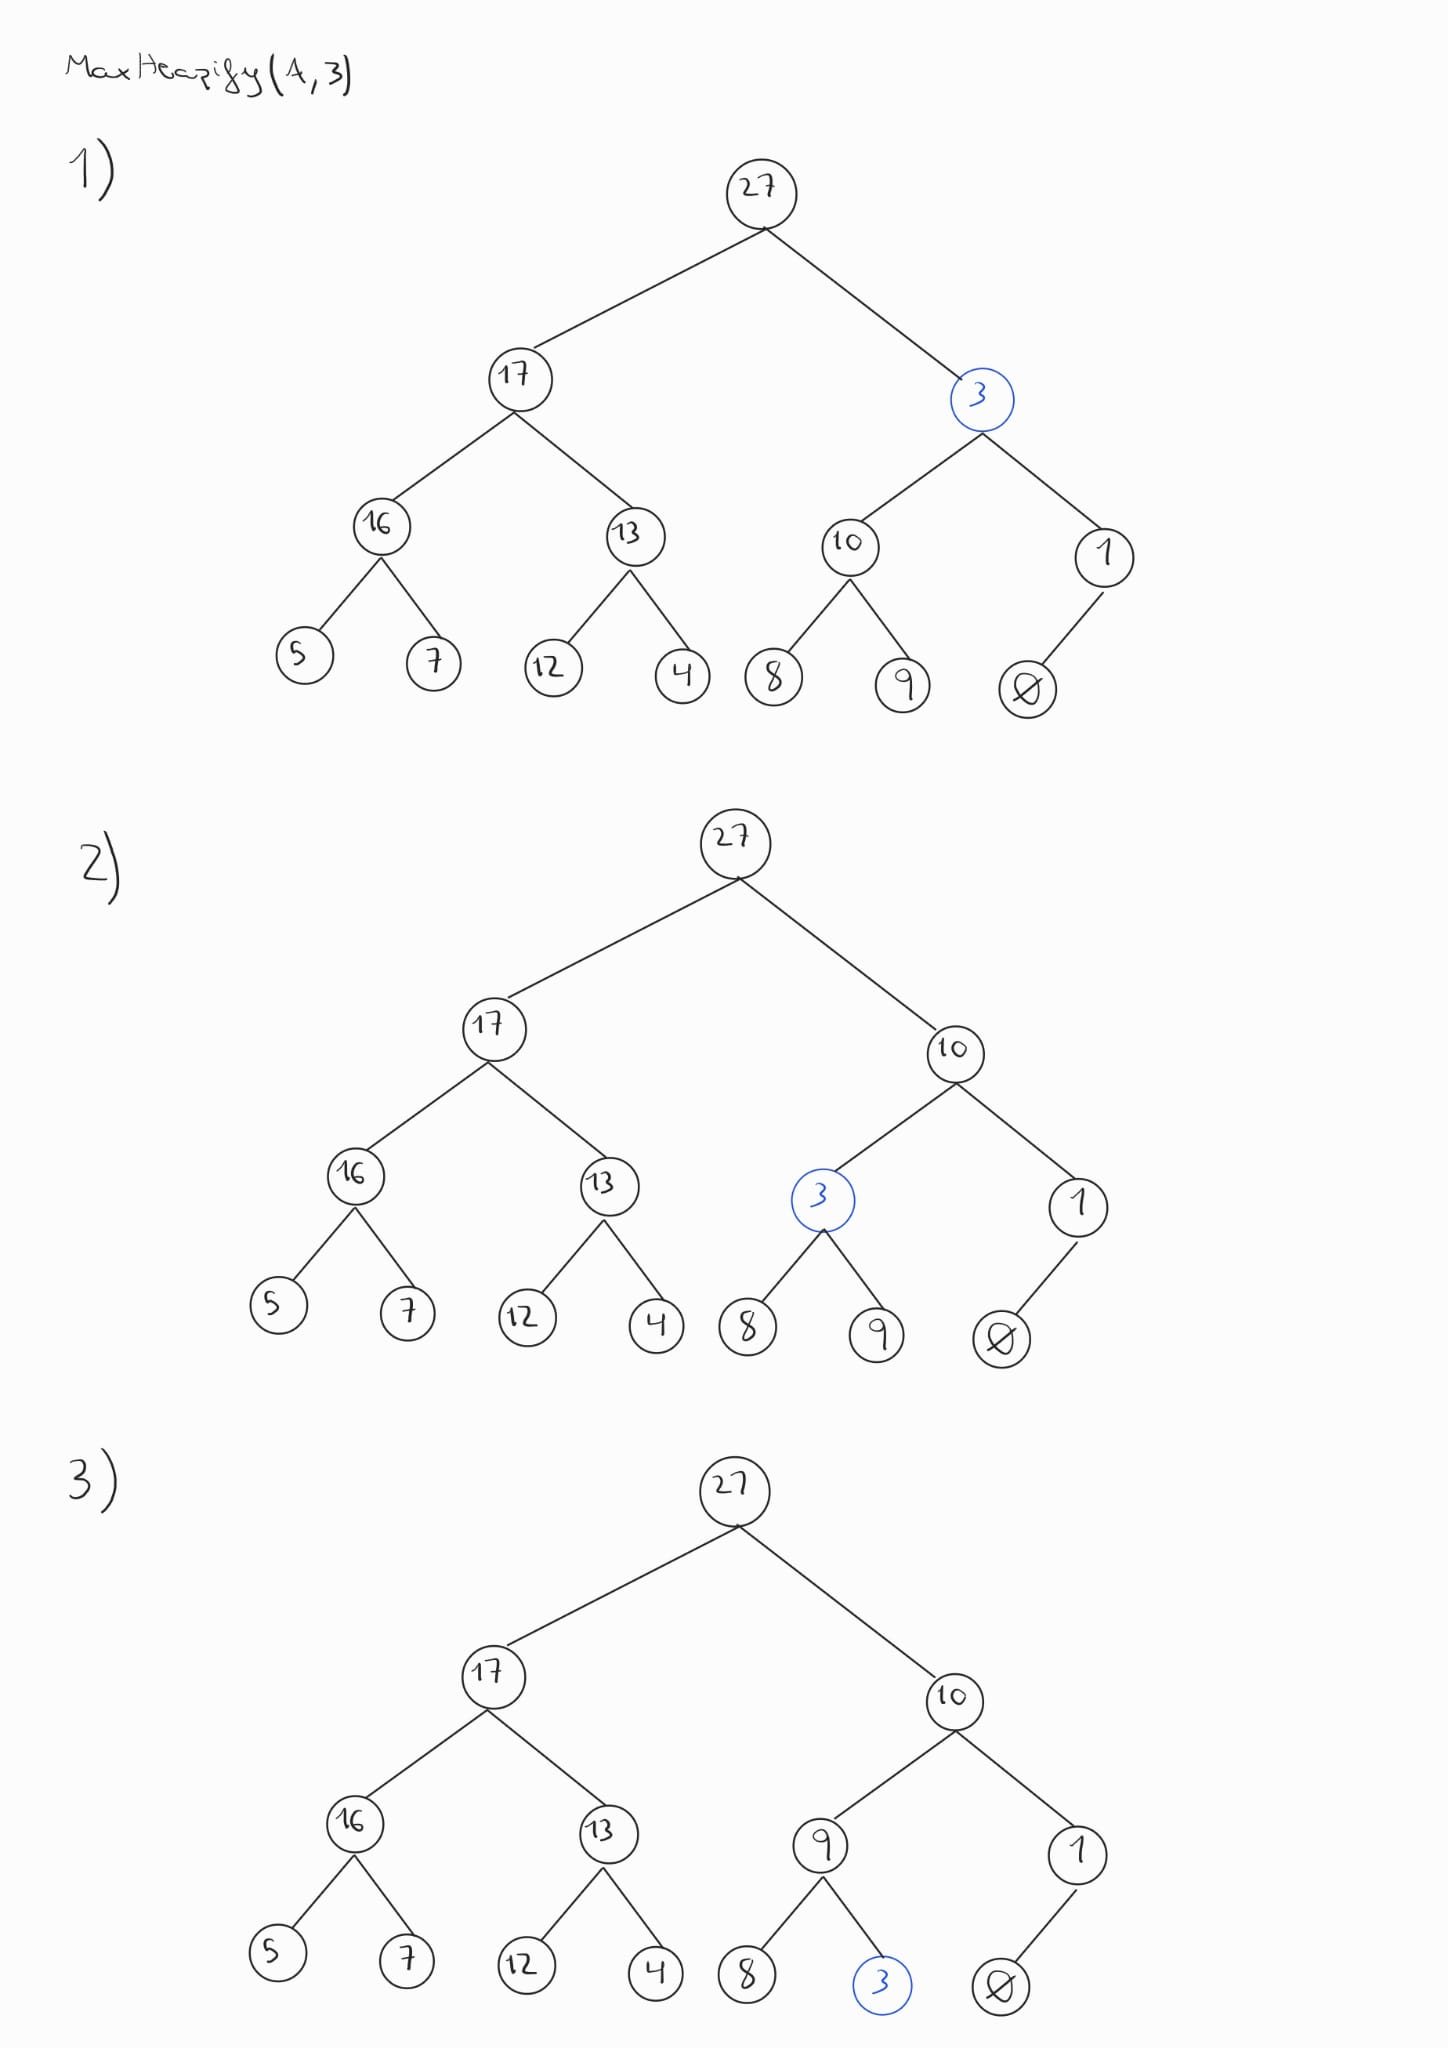
\includegraphics[scale=0.25]{Problem6_2_1.jpeg}
\end{figure}

\refstepcounter{exercise}
\textbf{Exercise 6.2-2)}:\\
Supose \(A_1\) and \(A_2\) are the childrens of the root. They are also the roots of another 
subtrees. We know they are balanced so one subtree can't have more nodes that the other subtree.
If one tree has more than \(\frac{2n}{3}\) nodes, the other one must have \(\frac{n}{3}\) and
that would violate the properties of the binary trees. 

The smallest possible value is \(\alpha = \frac{2}{3}\). 

\refstepcounter{exercise}
\textbf{Exercise 6.2-3)}:\\
The pseudocode used as reference is the one that appears on page 165.
It would be the same but only changing the conditions of the first 2 if. Also we can change
the variable name \(largest\) with \(lowest\)
The changes would be \(if l \leq A.heap_size and A[l] < A[i] then lowest = l\), on the other
if would be \(if r \leq A.heap_size and A[r] < A[lowest] then lowest = r\). The reamining
lines of the pseudocode would be the same.

\refstepcounter{exercise}
\textbf{Exercise 6.2-4)}:\\
it won't continue making recursive calls, because that mean the subtree on the root has the 
biggest value posible following the definition of max-heap.

\refstepcounter{exercise}
\textbf{Exercise 6.2-5)}:\\
Anything because from A.heap-size / 2 it's located all the leafs of the main tree. Due to 
that, any comparasions will be done.

\refstepcounter{exercise}
\textbf{Exercise 6.2-6)}:\\
Resolved on the file: \href{https://github.com/Graburr/Algorithms_CLRS_4ed_solutions/blob/main/chapter2/Sorting_and_Order_Statics/6.2-6.cpp}
{\textcolor{Blue}{6.2-6.cpp}}

\refstepcounter{exercise}
\textbf{Exercise 6.2-7)}:\\
Supose that you start from the root. Also supose that from the inmediate children of the 
root, it will be called recursively. As we are going down until reach a leaf, also we 
know a tree has \(\log_2 n \) levels in that case it's the same as the amount of time
the recursive call will be done. Due to that, the worst case is \(O(\log_2 n)\) as the 
sentence says.

\refstepcounter{exercise}
\textbf{Exercise 6.3-1)}:
\begin{figure}[h]
    \centering
    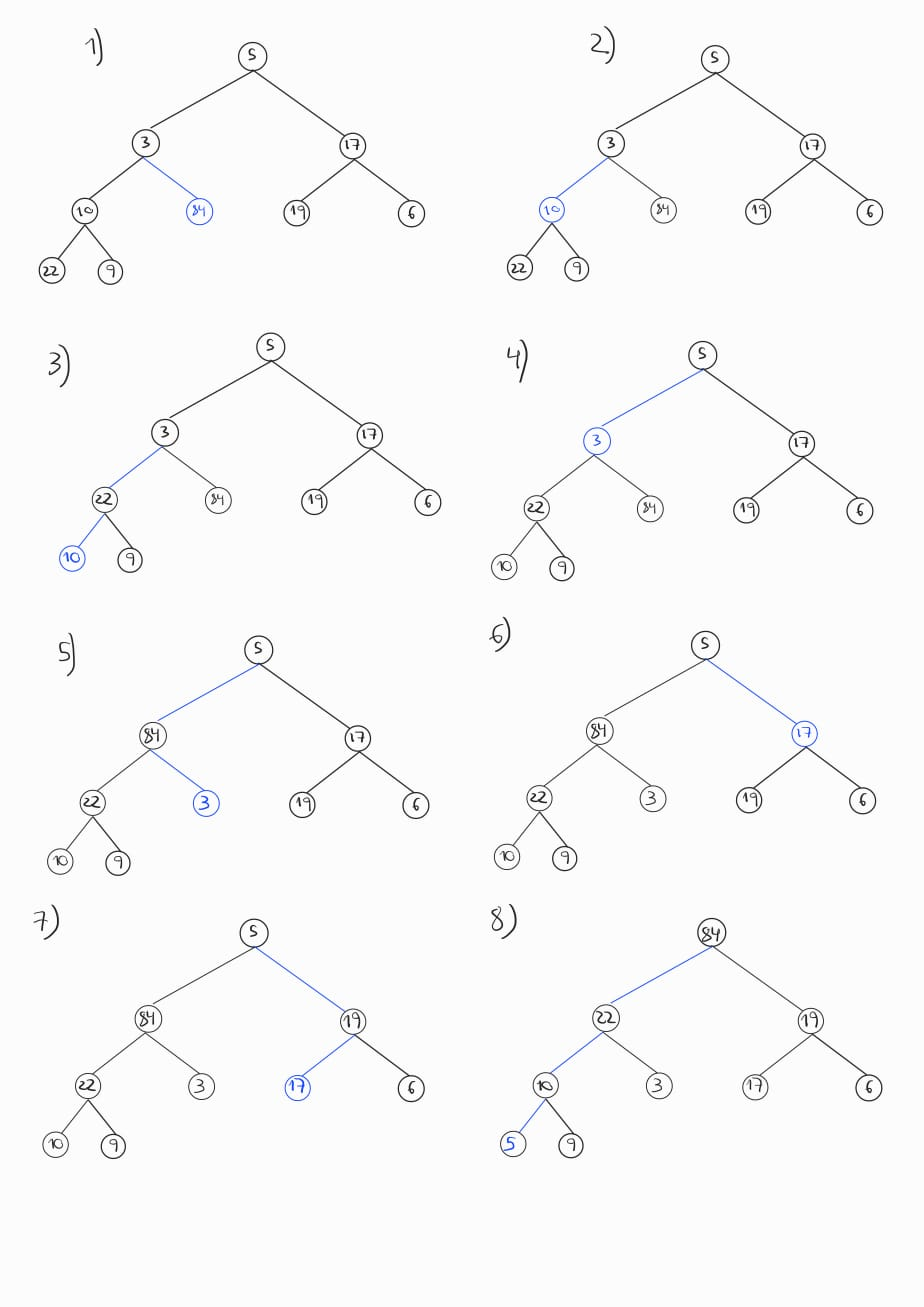
\includegraphics[scale=0.32]{Problem6_3_1.jpeg}
\end{figure}
\newpage

\refstepcounter{exercise}
\textbf{Exercise 6.3-2)}:
\[
\frac{n}{2^h} \geq \frac{1}{2} \quad \Rightarrow \quad n \geq \frac{1}{2} 2^h \quad
\Rightarrow \quad \log_2 n \geq h
\]
Because \(h\) is the height of the tree, and the height starts from 0, the result is:
\[
0 \leq h \leq \lfloor \log_2 n \rfloor 
\]

\refstepcounter{exercise}
\textbf{Exercise 6.3-3)}:\\
Doing from bootom-up you have guarantees that the lees posible subtree is ordered. Hence
on the fathers subtrees, when you order them you have guarantees that the child subtree
is ordered. While on the other way we cant guarantee that. 

\refstepcounter{exercise}
\textbf{Exercise 6.3-4)}:\\
We know that on each height on the tree, the numbers of elements got doubled. Also, the
number of elements in the heap, is at least \(n\) and the ttal number of elements are
\(2^h + 1\). Due to that the result is what the sentence is asking about proof.

\refstepcounter{exercise}
\textbf{Exercise 6.4-1)}:
\begin{figure}[h]
    \centering
    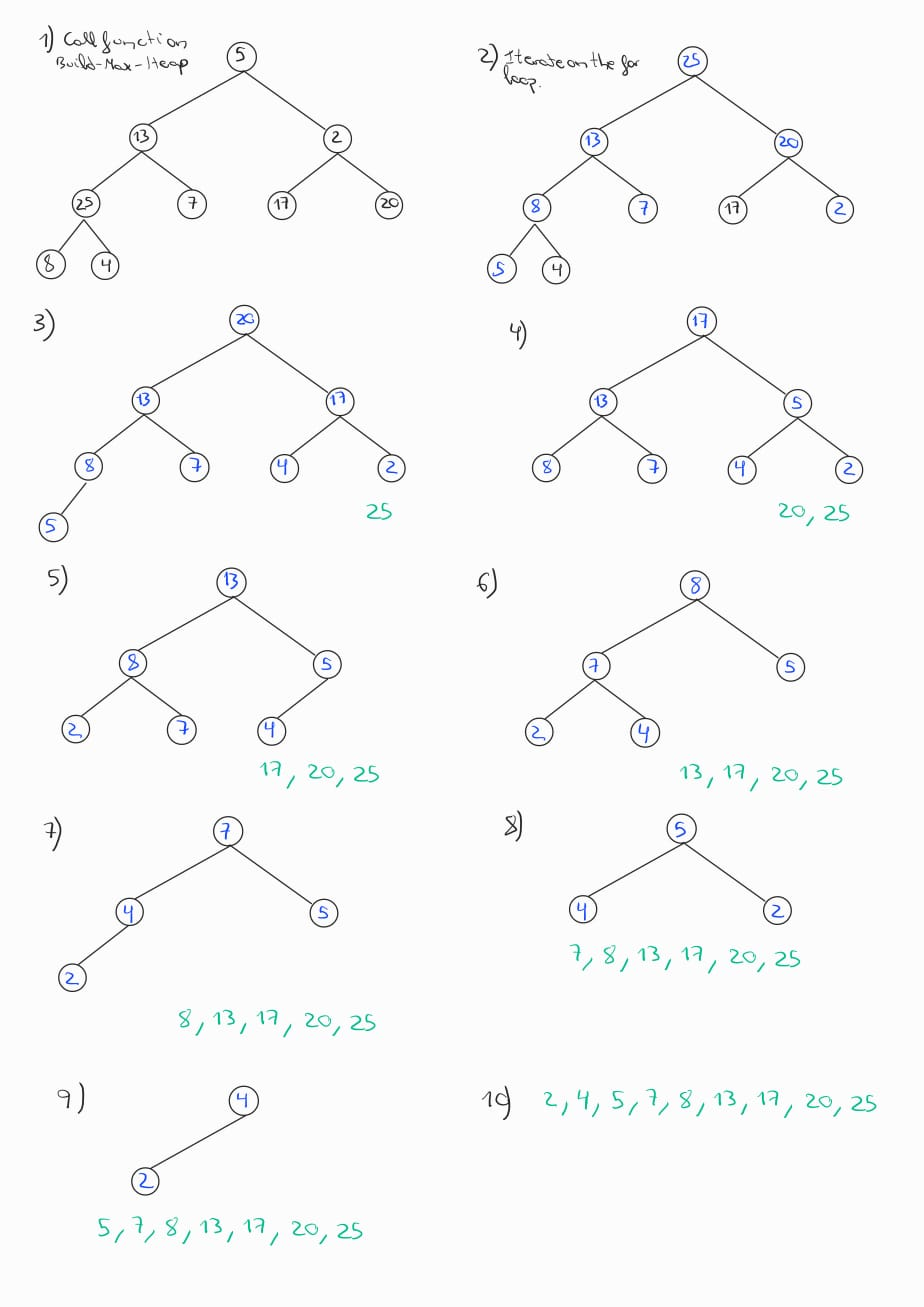
\includegraphics[scale=0.32]{Problem6_4_1.jpeg}
\end{figure}
\newpage

\refstepcounter{exercise}
\textbf{Exercise 6.4-2)}:\\
\textbf{Initialization:} At the start of the loop (before the first iteration), the
subarray \( A[1:n] \) is not sorted, but in the first iteration of the loop, the
\texttt{MaxHeapify} function is executed over the entire array, ensuring that the
array becomes a \textbf{max-heap}. Then, the largest element (at the root of the max-heap)
is placed in its final position, that is, at the last position of the array, ensuring
that the subarray \( A[1:n] \) contains the smallest elements, while \( A[n] \) contains
the largest element.

\textbf{Maintenance:} In each iteration of the loop, the following steps occur:

\begin{enumerate}
    \item The subarray \( A[1:i] \) is still a \textbf{max-heap} containing the \( i \)
    smallest elements of \( A[1:n] \).
    \item Then, the element at the root (the largest one) is moved to position \( i \).
    At this point, the subarray \( A[1:i-1] \) contains the \( i-1 \) smallest elements
    sorted (i.e., the largest ones).
    \item The subarray \( A[i:n] \) now contains largest elements sorted.
    \item The size of the heap is reduced by one (since the largest value has been placed
    in its correct position), and the \texttt{MaxHeapify} function is applied again to
    restore the heap property in the subarray \( A[1:i-1] \).
    \item This process repeats until the array is completely sorted.
\end{enumerate}

\textbf{Termination:} The loop terminates when \( i \) reaches 1, that is, when the
array is completely sorted. At the end of all iterations, the subarray \( A[1:n] \)
will be sorted in increasing order, and the max-heap property will have been maintained
at all times.

\refstepcounter{exercise}
\textbf{Exercise 6.4-3)}:\\
It would be \(\Omega(n \log_2 n)\) because on the inner loop it will always remove the largest
value, replace the root value with the less one, and then execute the function, it makes 
all time expend \(\Theta(n \log_2 n)\).

\refstepcounter{exercise}
\textbf{Exercise 6.4-4)}:\\
Explained on the before exercise. Same logic as this.

\refstepcounter{exercise}
\textbf{Exercise 6.4-5)}:\\
It's the same explaination as the 2 before exercise. In this case the first function outside
the loop could be in the average time, but the inner loop will be always \(\Theta(n \log_2 n)\).

\refstepcounter{exercise}
\textbf{Exercise 6.5-1)}:\\
It just extract the element at the first position (because it's the biggest one). Then do
the swap as HeapSort with the last element, to move at the first position the next biggest
element.

\refstepcounter{exercise}
\textbf{Exercise 6.5-2)}:\\
Is added on the index with the value of textit{heap\_size}, then when calling the function
\textit{Max\_heap\_increase\_key}, it will compare the value of the key with its parent keys,
and will change the position if the parent key is less than the new key to be inserted.
When that condition is not satisfied (or the new key reaches the root), it will end the
procedure of insert because it will be inserted in the correct position.

\refstepcounter{exercise}
\textbf{Exercise 6.5-3)}:\\
the functions \textit{Min-Heap-Minimum} and \textit{Min-Heap-Exctract-Min} are the same as
the max version because the min-heap will have the least value possible on the root. On the
\textit{Min-Heap-Decrease-Key}, the only change needed is at the while condition. The max
version has \(while i > 0 \textit{ and } A[Parent(i)].key < A[i].key\), while the min version 
would be \(while i > 0 \textit{ and } A[Parent(i)].key > A[i].key\), changing the less operator
by the greater operator. The change needed on \textit{Min-Heap-Insert} is \(-\infty\) by
\(\infty\). 

\refstepcounter{exercise}
\textbf{Exercise 6.5-4)}:
\begin{algorithm}[H]
    \caption{MAX-HEAP-DECREASE-KEY($A$, $i$, $k$)}
    \begin{algorithmic}[1]
        \State \textbf{Input:} A max-heap \(A\), index \(i\), new key value \(k\) with \(k \le A[i].\text{key}\)
        \State \textbf{Output:} Updated max-heap with \(A[i].\text{key} = k\)
        \If{\(k > A[i].\text{key}\)}
            \State \textbf{error} "new key is larger than current key"
        \EndIf
        \State \(A[i].\text{key} \gets k\)
        \State \textbf{call} MAX-HEAPIFY\((A,i)\)
    \end{algorithmic}
\end{algorithm}

\refstepcounter{exercise}
\textbf{Exercise 6.5-5)}:\\
It could contain any value. Also it could take a value larger than the key and it will cause 
an error, so adding that value, we make sure that no error will occur.

\refstepcounter{exercise}
\textbf{Exercise 6.5-6)}:\\
\textit{Max-Heapify} "sinks" the element correcting the errors at the directoin to their 
childs. The violation that can happens is that the new key value is larger than it's father,
o fix that it wuld need to buuble up. So with the function \textit{Max-Heapify} this can't
be done, because it asume that all subtrees are max-heaps. Therefore, it couldn't be that
case and it could be positioned in a bad position.

\refstepcounter{exercise}
\textbf{Exercise 6.5-7)}:\\
\textbf{Initialization:} At the beggining, we have a new element in a leaf, the a and b
conditions are true but the c condition can occur with the new element inserted.

\textbf{Maintenance:} On each iteration it will interchange the child with the father if the
father has lees value key than the child. Therefore the condition a and b will be satisfied
on each iteration if that change is done. But the biggest subtrees couldnt be satisfied leading
to the option c. Therefore it will be changing all time with their fathers until satisfies
the condition that \(A[1:A.heap-size]\) satisfies the max-heap property.

\textbf{Termination:} When the while loops end. The condition a and b will be true for all
possible subtrees, but the condition c wont' be satisfied because the start invariant which
says \(A[1:A.heap-size]\) satisfies the max-heap property, it will be true to every subtree.
Hence it's satisfies the condition when the first call is done to that function.

\refstepcounter{exercise}
\textbf{Exercise 6.5-8)}:\\
The idea is to move to the bottom just the key values, it will make only 1 assigment. Then
when you need to retrieve the objects with that values, you only need to retrieve the key
value and find which object is associated with that key value.

\refstepcounter{exercise}
\textbf{Exercise 6.5-9)}:\\
To each element that is inserted, you start associating a key with the biggest possible
value. Doing that you make sure that the first value inserted it will be the first value
to be extracted when the function \textit{Max-Heap-Extract-Max} is called (is the analogous)
function for the pop function of a queue.

\refstepcounter{exercise}
\textbf{Exercise 6.5-10)}:\\
Replace the node to be deleted witht he last node of the heap. Update the size of the heap
(incrementing it by 1), and then call \textit{Max-Heapify} to sort again the elements.
This function called has a runtime of \(O(\log_2 n)\) as we explained at exercise done before.
Due to that this function has a complexity of \(O(\log_2 n)\) too.

\subsection{QuickSort}
\setcounter{exercise}{0}

\refstepcounter{exercise}
\textbf{Exercise 7.1-1)}:
\begin{align*}
    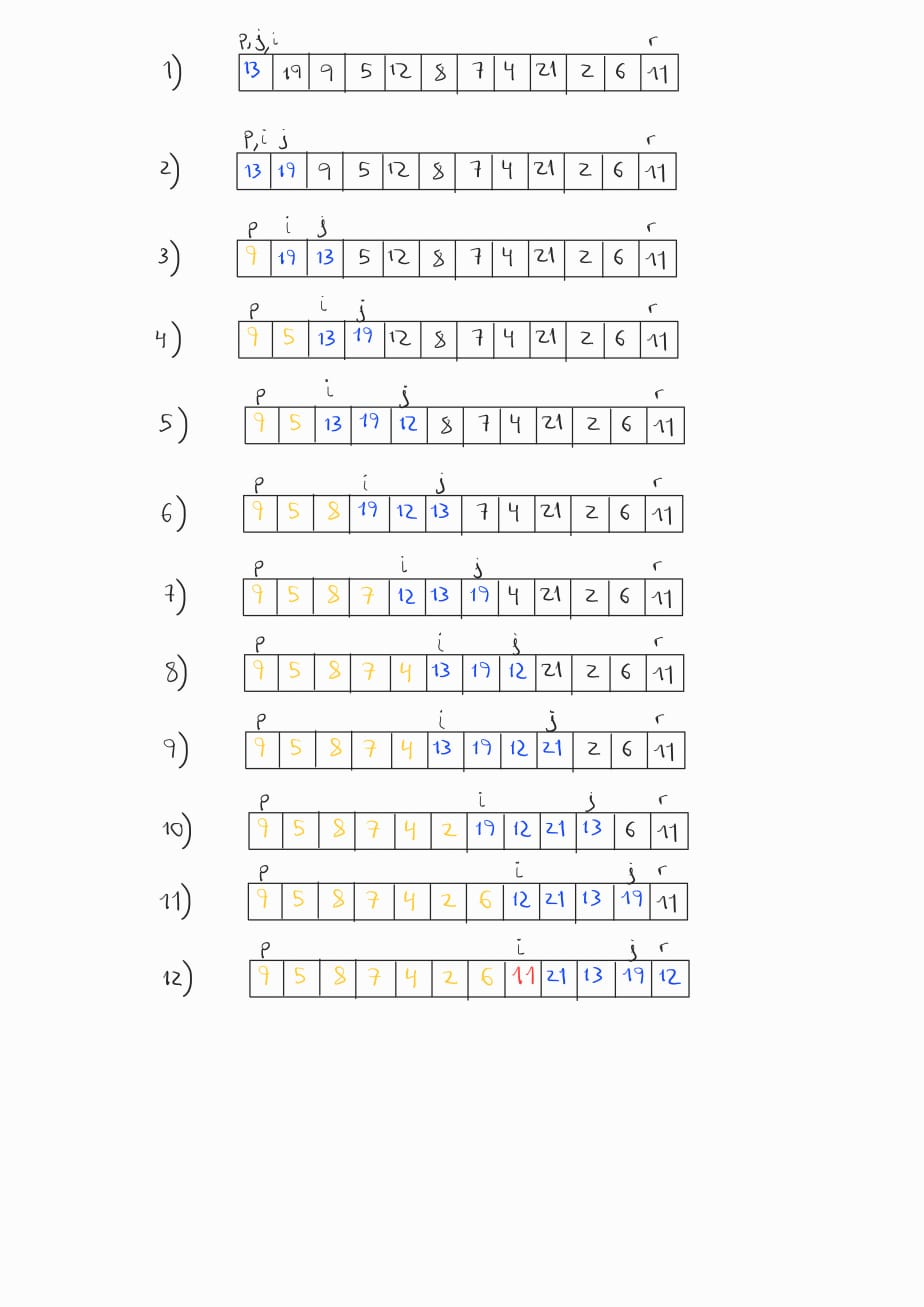
\includegraphics[scale=0.5]{Problem7_1_1.jpeg}
\end{align*}
\newpage

\refstepcounter{exercise}
\textbf{Exercise 7.1-2)}:\\
It returns the last value of the array, in other words, q = r. To fix that we could introduce
a boolean value initialized to false. If any swap happends, set that boolean to true. At the
end, if the boolean is false, return \(\lfloor (p + r)/2 \rfloor\). 

\refstepcounter{exercise}
\textbf{Exercise 7.1-3)}:\\
At the beggining, \(p = 1\) and \(r = n\) where n it's the size of the array. Due to that,
the for loop iterates n elements of the array.

\refstepcounter{exercise}
\textbf{Exercise 7.1-4)}:\\
Change the \(if A[j] \leq x\) by \(if A[j] > x\) To sort in decrease order.

\refstepcounter{exercise}
\textbf{Exercise 7.2-1)}:\\
Induction hypotesis used is \(T(m) = cm^2\). \(T(n) \leq c(n - 1)^2 + kn \leq cn^2\). Due 
to that, the solution is \(T(n) = cn^2\).

\refstepcounter{exercise}
\textbf{Exercise 7.2-2)}:\\
We are on the case \textit{a} of figure 7.5. Then \(T(n) = T(n - 1) + \Theta(n) = \Theta(n^2)\).

\refstepcounter{exercise}
\textbf{Exercise 7.2-3)}:\\
Because all elements are less than the pivot, we are on the partition case of the exercise
7.2-1 because 1 subarray will be empty and the other one will have \(n - 1\) values. Hence
the running time is \(\Theta(n^2)\).

\refstepcounter{exercise}
\textbf{Exercise 7.2-4)}:\\
We have to remaind that Insertion Sort is good when all elements are almost sorted. In that
case insertion sort is \(O(n + d)\) where \textit{d} is too small. Therefore the running
time is \(O(n)\). While QuickSort, have to select the pivot, then compare the elements,
move them depends of the pivot, etc. Due to that, Insertion Sort is \(O(n \log_2 n)\) which
is slower than \(O(n)\).

\refstepcounter{exercise}
\textbf{Exercise 7.2-5)}:\\
This exercise is the same as the Figure 7.4 but with constant values. One array will be
partitioned by the contstant \(\alpha\) and the other one by \(\beta\). Because \(\beta\)
is bigger, this partition will end later than \(\alpha\). However each one will have a depth
\(\log_{1 / \alpha} n\) and the other one \(\log_{1 / \beta} n\). 

\refstepcounter{exercise}
\textbf{Exercise 7.2-6)}:\\
Assume we have an array of \( n \) distinct elements where all permutations are equally 
likely.
For the partition to be at least as balanced as \( (1-\alpha):\alpha \) (with \(0 < \alpha \le \frac{1}{2}\)), the pivot must be chosen among the elements ranked between
\[
\lceil \alpha n \rceil \quad \text{and} \quad \lfloor (1-\alpha) n \rfloor.
\]
The number of such “good” pivot positions is approximately
\[
\lfloor (1-\alpha)n \rfloor - \lceil \alpha n \rceil + 1 \approx (1-2\alpha)n.
\]
Since each element is equally likely to be chosen as the pivot, the probability of a 
balanced split is
\[
\frac{(1-2\alpha)n}{n} = 1-2\alpha.
\]

\refstepcounter{exercise}
\textbf{Exercise 7.3-1)}:\\
Because for the same inputs on each execution, the result it isn't the same because there is
a random factor on the algorithm. 

\refstepcounter{exercise}
\textbf{Exercise 7.3-2)}:\\
The best one is: \(T(n) = 2T(\frac{n}{2}) + O(1) = O(n)\).

The worst is : \(T(n) = T(n - 1) + O(1) = O(n)\).

\subsection{Sorting in Linear Time}
\setcounter{exercise}{0}

\refstepcounter{exercise}
\textbf{Exercise 8.1-1)}:\\
Following the theorem 8.1, the possible depth is \(\log_2 h\).

\refstepcounter{exercise}
\textbf{Exercise 8.1-3)}:\\
Supose for the sake of contradiction, that there exists a comparison
sort that runs in linear time, say \(O(n)\), on at least half of the inputs.
That is, there exists a constant \(c>0\) such that for at least
\(\frac{n!}{2}\) inputs,
\[
T(n) \le c\, n.
\]

Let the running time on the remaining inputs be at most \(O(n\log n)\)
(since no algorithm can beat the \(\Omega(n\log n)\) worst-case lower bound).
Then the overall average running time would be bounded by
\[
\frac{1}{n!}\Biggl(\frac{n!}{2}\cdot c\, n + \frac{n!}{2}\cdot O(n\log n)\Biggr)
=\frac{1}{2}\cdot c\, n+\frac{1}{2}\cdot O(n\log n)=O(n\log n).
\]

This suggests that the average running time is only a constant factor
times \(n\log n\). However, the decision tree lower bound implies that almost
all inputs (i.e., a non-negligible fraction) must incur \(\Omega(n\log n)\)
comparisons to reach the lower bound. In other words, if half the inputs were as
fast as \(O(n)\), the average could not be as high as \(\Omega(n\log n)\).

Thus, no comparison sort can run in \(O(n)\) time on at least half of the
\(n!\) inputs.

\textbf{What about a fraction \(1/n\) or \(1/2^n\)?}\\[1mm]
If an algorithm were to run in linear time on a fraction \(1/n\) (or \(1/2^n\))
of the inputs, the contribution of those inputs to the overall average would be
\[
\frac{1}{n!}\Biggl(\frac{n!}{n}\cdot O(n)\Biggr)=O(1)
\quad \text{(or even smaller for }1/2^n\text{)},
\]
while the remaining inputs (which form almost all of the \(n!\) inputs) must
still incur \(\Omega(n\log n)\) comparisons. Therefore, the overall average 
remains \(\Omega(n\log n)\).

\refstepcounter{exercise}
\textbf{Exercise 8.1-4)}:\\
We show that any comparison sort must take 
\(\Omega(n\log n)\) comparisons even for inputs that satisfy the following 
promise: For every index \(i\) with \(i \bmod 4 = 0\), the element that is 
initially at position \(i\) will, after sorting, appear in one of the positions 
\(i-1\), \(i\), or \(i+1\). For the remaining positions (those with \(i \bmod 4 
\neq 0\)), no constraint is given.

Consider the set \(S\) of all input orders consistent with this promise. Note 
that the elements in positions \(i\) with \(i \bmod 4 \neq 0\) may appear in 
any order. Thus, there are at least \((3n/4)!\) possible orderings for these 
elements. By Stirling's approximation, we have
\[
\log_2\bigl((3n/4)!\bigr)=\Omega(n\log n).
\]

Since any comparison sort must distinguish among all these distinct inputs, 
its decision tree must have at least \(\Omega(2^{\,n\log n})\) leaves. This 
implies that in the worst case the sort must perform at least 
\(\Omega(n\log n)\) comparisons.

\newpage
\refstepcounter{exercise}
\textbf{Exercise 8.2-1)}:
\begin{figure}[h]
    \centering
    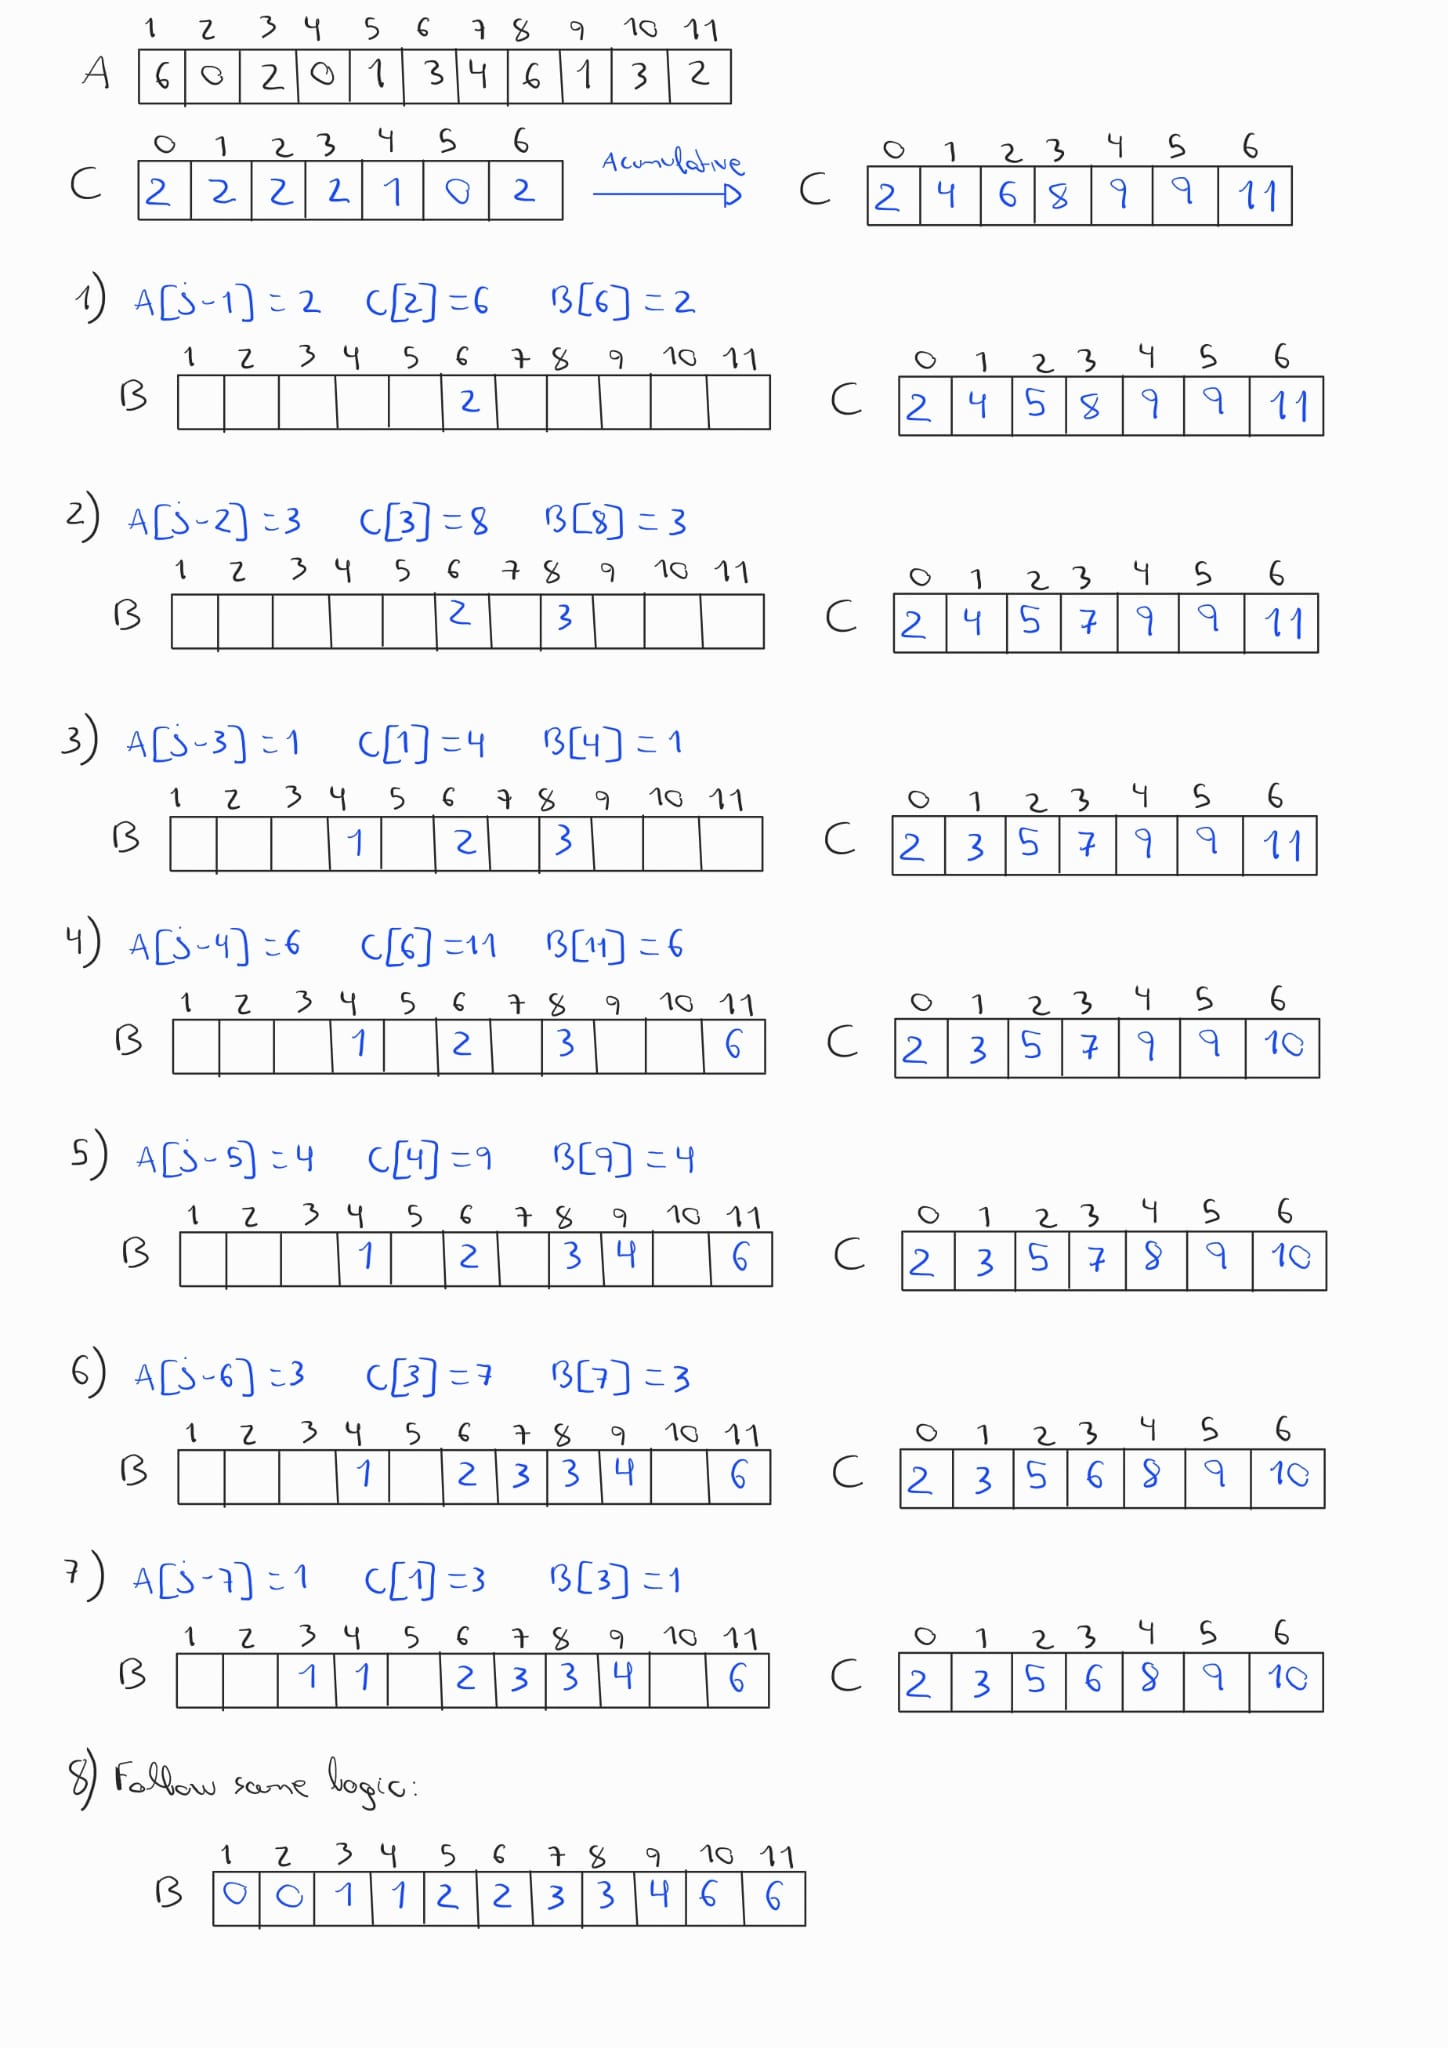
\includegraphics[scale=0.25]{Problem8_2_1.jpeg}
\end{figure}

\refstepcounter{exercise}
\textbf{Exercise 8.2-2)}:\\
It's stable because u start order them on B from the final, so the last values added on the
vector A, is suposed to be on the last position. If vector A has two equals values, the first
one that appear starting from the final of the array, is placed at the position \textit{k},
while the next element with the same value, will be placed at \(k - 1\), making that algorithm
stable.

\refstepcounter{exercise}
\textbf{Exercise 8.2-3)}:\\
In this case the first value inserted on the array will be on a position \textit{k} on the
output array. The second time that appear an element with the same value, will be situated
on \(k - 1\) changing the order when the elements were inserted. In that case the 
\textbf{stable} property is not guarantee.

\refstepcounter{exercise}
\textbf{Exercise 8.2-4)}:\\
\textbf{Initialization:} \\
Before the loop starts, the array $C$ has been computed such that $C[i]$ stores 
the position where the last element of value $i$ should be placed in $B$. 
Since no elements have been copied yet, the invariant holds.

\textbf{Maintenance:} \\
At the start of each iteration, the last unplaced element in $A$ of value $i$ 
is correctly positioned in $B[C[i]]$. After placing it, $C[i]$ is decremented, 
ensuring the next occurrence of $i$ is placed correctly in the next iteration. 
Thus, the invariant holds throughout the loop.

\textbf{Termination:} \\
When the loop ends, all elements from $A$ have been placed in $B$ in a stable order. 
Since every element was placed in its correct position using $C$, and $C[i]$ was 
decremented correctly, $B$ is now a sorted version of $A$. 

Thus, the loop invariant holds, proving the correctness of COUNTING-SORT.

\refstepcounter{exercise}
\textbf{Exercise 8.2-5)}:\\
\begin{algorithm}
    \caption{Counting Sort In-Place}
    \begin{algorithmic}[1]
    \Require Array $A$ of size $n$, maximum value $k$
    \Ensure Sorted array $A$
    \State Initialize array $C$ of size $k$ with zeros
    \For{$j = 0$ to $n - 1$}
        \State $C[A[j]] \gets C[A[j]] + 1$
    \EndFor
    \State $index \gets 0$
    \For{$i = 0$ to $k - 1$}
        \While{$C[i] > 0$}
            \State $A[index] \gets i$
            \State $index \gets index + 1$
            \State $C[i] \gets C[i] - 1$
        \EndWhile
    \EndFor
    \end{algorithmic}
\end{algorithm}

\refstepcounter{exercise}
\textbf{Exercise 8.2-6)}:\\
It's just consist of making the first 2 for loops of counting sort. Then when it gives 
\(a\) and \(b\), just substract and return \(C[b] - C[a - 1]\) to give the answer to that 
question.

\newpage
\refstepcounter{exercise}
\textbf{Exercise 8.2-7)}:\\
\begin{algorithm}
    \caption{Counting Sort for Numbers with Fractional Parts}
    \begin{algorithmic}[1]
        \Require Array $A$ of $n$ numbers in range $[0, k]$ with at most $d$ decimal digits
        \Ensure Sorted array $A$ in $O(n + 10^d k)$ time
        \State Multiply each $A[i]$ by $10^d$ to convert to an integer
        \State Find max value $k' \gets 10^d k$
        \State Initialize count array $C$ of size $k' + 1$ with zeros
        \For{$j \gets 0$ to $n - 1$}
        \State $C[A[j]] \gets C[A[j]] + 1$
        \EndFor
        \For{$i \gets 1$ to $k'$}
        \State $C[i] \gets C[i] + C[i-1]$
        \EndFor
        \For{$j \gets n - 1$ to $0$}
        \State Place $A[j]$ in sorted position using $C$
        \State $C[A[j]] \gets C[A[j]] - 1$
        \EndFor
        \State Divide each $A[i]$ by $10^d$ to restore original scale
    \end{algorithmic}
\end{algorithm}

\refstepcounter{exercise}
\textbf{Exercise 8.3-1)}:
\begin{figure}[h]
    \centering
    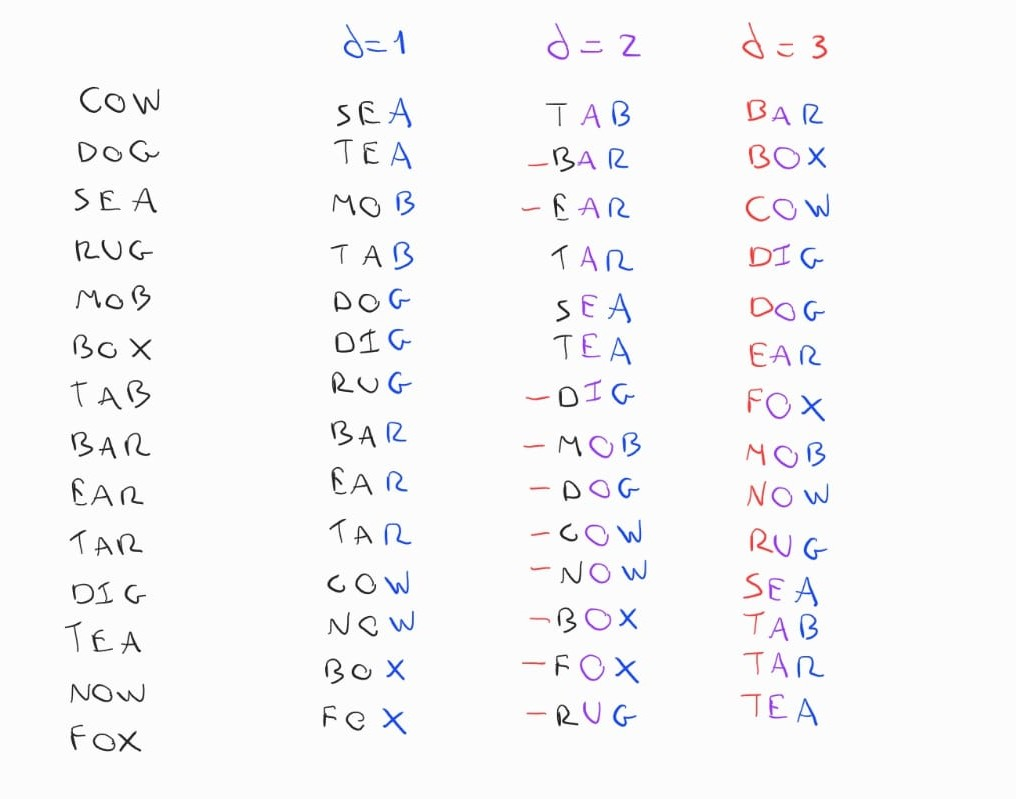
\includegraphics[scale=0.3]{Problem8_3_1.jpeg}
\end{figure}

\refstepcounter{exercise}
\textbf{Exercise 8.3-2)}:\\
Insertion sort, merge sort are stables. On the other hand, heapsort and QuickSort aren't 
stables.

\refstepcounter{exercise}
\textbf{Exercise 8.3-3)}:\\
\textbf{Base Case:} For $d=1$, radix sort uses a stable sort on one digit.
Thus, the array is correctly sorted by that digit.\\[1ex]
\textbf{Inductive Hypothesis:} Assume that after sorting by $d-1$ digits,
the array is correctly sorted with respect to the $d-1$ least significant 
digits.\\[1ex]
\textbf{Inductive Step:} Now, sort by the $d$th digit using a stable sort.
Because the sort is stable, elements with equal $d$th digits retain their
relative order from the previous pass (sorted by the lower $d-1$ digits).
Thus, the entire array becomes sorted by all $d$ digits.\\[1ex]
\textbf{Conclusion:} By induction, radix sort sorts the array correctly.
The proof requires the stability assumption in the inductive step,
to preserve the order established by the lower digits when sorting by
a higher digit.

\refstepcounter{exercise}
\textbf{Exercise 8.3-5)}:\\
It could be make using radix sort because they are positive numbers. We need to know if
the \(n^3\) are dozens, hundreds, to set the value d for the radix sort algorithm. Then
apply radix sort to sort it in \(O(d(n))\). Keep in mind that values that have less length
that \(n^3\), will be evaluated to 0 when their length is exceded, making them be at the
first position.

\refstepcounter{exercise}
\textbf{Exercise 8.3-6)}:\\
It will require \textit{d} passes. In the worst case there will be 10 piles of card at the
same time.

\subsection{Medians and Order Statics}
\setcounter{exercise}{0}

\refstepcounter{exercise}
\textbf{Exercise 9.1-1)}:\\
Solution on cpp: \href{https://github.com/Graburr/Algorithms_CLRS_4ed_solutions/blob/main/chapter2/Medians_and_Order_Statics/Exercise9.1_1.cpp}
{\textcolor{Blue}{Exercise9.1\_1.cpp}}.

\refstepcounter{exercise}
\textbf{Exercise 9.1-2)}:\\
As explained before it's necesary \(3\lfloor\frac{n}{2}\rfloor\) if it's odd, or \(3(n-2)/2\)
if it's even.

\refstepcounter{exercise}
\textbf{Exercise 9.1-3)}:\\
To determine the fastest horse need \(\frac{25}{n} + 1\) where \(n\) it's the amount of horses
that race at a time. It will need also the same, to take the 3 fastest one. Instead of only
store the fastest one on the sixth race, it will need to store the 3 best horses on the sixth
race.

\refstepcounter{exercise}
\textbf{Exercise 9.1-4)}:\\
Each pair requires 1 comparison to find both the local maximum and minimum.  
After pairing, you have \( \frac{n}{2} \) maximum candidates and \( \frac{n}{2} \) minimums.  
For odd \(n\), one extra comparison is needed for the unpaired element.  
Next, you need \( \frac{n}{2} - 1 \) comparisons to find the overall maximum.  
Similarly, \( \frac{n}{2} - 1 \) comparisons are required to find the minimum.  
Thus, the total number of comparisons is \( \left\lceil \frac{3n}{2} \right\rceil - 2 \).  
This is the lower bound for the number of comparisons in the worst case.

\section{Data Structures}

\subsection{Elementary Data Structures}
The part of arrays, linked list, queues and stacks, I didn't made any exercise because I
saw this data structures a lot throughout computer science leasons and other books.
\setcounter{exercise}{0}


\newpage
\refstepcounter{exercise}
\textbf{Exercise 10.3-1)}:
\begin{figure*}[h]
    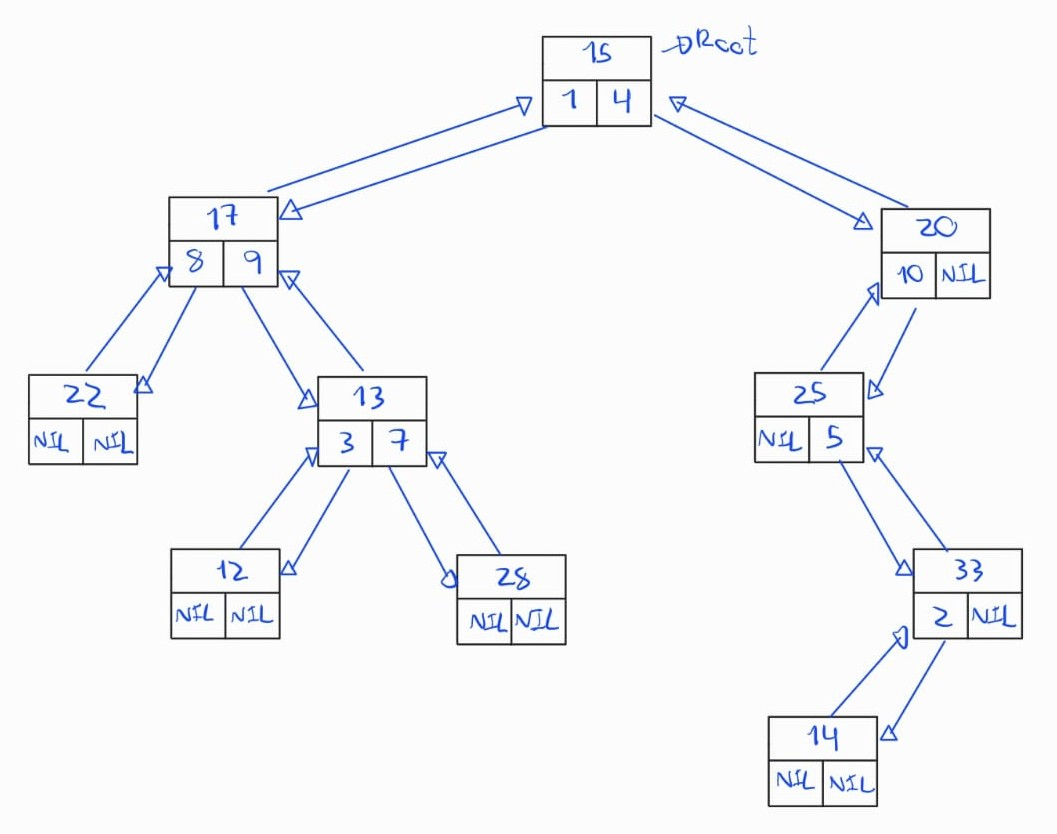
\includegraphics[scale=0.3]{Problem10_3_1.jpeg}
    \centering
\end{figure*}

\refstepcounter{exercise}
\textbf{Exercise 10.3-2)}:\\
Resolved on \href{https://github.com/Graburr/Algorithms_CLRS_4ed_solutions/tree/main/chapter3/Problem10_3_2.cpp}
{\textcolor{Blue}{Problem10\_3\_2.cpp}}.

\refstepcounter{exercise}
\textbf{Exercise 10.3-3)}:\\
Resolved on \href{https://github.com/Graburr/Algorithms_CLRS_4ed_solutions/tree/main/chapter3/Problem10_3_3.cpp}
{\textcolor{Blue}{Problem10\_3\_3.cpp}}.

\refstepcounter{exercise}
\textbf{Exercise 10.3-4)}:\\
Resolved on \href{https://github.com/Graburr/Algorithms_CLRS_4ed_solutions/tree/main/chapter3/Problem10_3_4.cpp}
{\textcolor{Blue}{Problem10\_3\_4.cpp}}.

\refstepcounter{exercise}
\textbf{Exercise 10.3-5)}:\\
Resolved on \href{https://github.com/Graburr/Algorithms_CLRS_4ed_solutions/tree/main/chapter3/Problem10_3_5.cpp}
{\textcolor{Blue}{Problem10\_3\_5.cpp}}.



\end{document}
